% numerical.tex

\cleardoublepage
\chapter{Optimised Trajectory Including Fly-Back}\label{chapter:Flyback}


This chapter presents the maximum payload-to-orbit optimised trajectory of the rocket-scramjet-rocket launch system, with the fly-back of the SPARTAN included within the optimal trajectory calculation. 
Flying back the SPARTAN for landing at the initial launch site is one of the primary enabling factors in the cost efficient operation of the launch system. If the SPARTAN is launched onto a trajectory from which it is not able to fly-back, it must perform a downrange landing, likely at an Indonesian airfield when launched northerly from north Australia. This would necessitate transporting the SPARTAN back to Australia, a costly and time consuming process, as well as organising international landing facilities. 
Flying back the SPARTAN removes the need for costly transportation from a downrange launch site, and allows for rapid refurbishment and re-use, as the SPARTAN returns during the launch process.
In addition, if a launch site is used from which there is no downrange land mass, the SPARTAN must necessarily fly-back to the initial launch site. 

The fly-back of the SPARTAN requires turning-around the SPARTAN after third stage separation, covering the necessary ground distance for return, and decelerating to reduce the speed of the SPARTAN to landing approach velocity, while maintaining a suitable descent angle to allow for a controlled approach. 
The return of the SPARTAN to the initial launch site is included in the optimisation process to asses whether it is possible for fly-back of the SPARTAN to be achieved as a part of the launch process, and to maximise the overall payload-to-orbit efficiency of the launch system. This is compared to the optimised, maximum payload-to-orbit trajectory without fly-back (detailed in Chapter \ref{chapter:Ascent}) to assess the detrimental effects of the fly-back on the performance of the launch system. 
A sensitivity analysis is conducted, in a similar fashion to Chapter \ref{chapter:Ascent}. 
This sensitivity analysis allows the influence of the fly-back of the SPARTAN on the design sensitivities of the launch system to be assessed.


\section{Case 11: Combined SPARTAN Ascent-Descent \& Third Stage}
\begin{table}[ht]
	\centering
\begin{tabular}{l c } 
	\hline \textbf{Trajectory Condition}
	&Value 
	\\
	\hline \textbf{Payload to Orbit (kg)}
	& \textbf{\PayloadToOrbitStandard}
	\\
	\textbf{Total $\eta_{exergy}$ (\%)}
	& \textbf{\totalExergyEffStandard}
	\\
	\hline 
	\textbf{1$^{st}$ Stage $\eta_{exergy}$ (\%)}
	& \textbf{\firstExergyEffStandard}
	\\

	\textbf{Separation Alt, 1$\rightarrow$2 (km)}
	& \firstsecondSeparationAltStandard
	\\
	\textbf{Separation v, 1$\rightarrow$2 (m/s)}
	& \firstsecondSeparationvStandard
	\\
	\textbf{Separation $\gamma$, 1$\rightarrow$2 (deg)}
	& \firstsecondSeparationgammaStandard
	\\
	\hline 
	\textbf{2$^{nd}$ Stage $\eta_{exergy}$ (\%)}
	& \textbf{\secondExergyEffStandard}
	\\

	\textbf{Separation Alt, 2$\rightarrow$3 (km)}
	& \secondthirdSeparationAltStandard
	\\
	\textbf{Separation $v$, 2$\rightarrow$3 (m/s)}
	& \secondthirdSeparationvStandard
	\\
	\textbf{Separation $\gamma$, 2$\rightarrow$3 (deg)}
	& \secondthirdSeparationgammaStandard
	\\
	\textbf{2$^{nd}$ Stage Flight Time (s)}
	& \secondFlightTimeStandard
	\\
	\textbf{2$^{nd}$ Stage Distance Flown (km)}
	& \SecondDistStandard
	\\
	\textbf{2$^{nd}$ Stage Return Fuel (kg)}
	& \returnFuelStandard
	\\
	\textbf{2$^{nd}$ Stage Return Distance (km)}
	& \returnDistStandard
	\\
	\hline 
	\textbf{3$^{rd}$ Stage $\eta_{exergy}$ (\%)}
	& \textbf{\thirddExergyEffStandard}
	\\

	\textbf{3$^{rd}$ Stage $t$, $q >$ 5kpa (s)}
	& \thirdqOverFiveStandard
	\\
	\textbf{3$^{rd}$ Stage max $\alpha$ (deg)}
	& \thirdmaxAoAStandard
	\\
	\textbf{3$^{rd}$ Stage Fuel Mass (kg)}
	& \thirdmFuelStandard
	\\
	\hline 
\end{tabular} 
\caption{Selected trajectory conditions for a maximum payload-to-orbit trajectory including SPARTAN fly-back (Case 11).}
\end{table}

LODESTAR is used to optimise the trajectory of the rocket-scramjet-rocket launch system, including the return of the SPARTAN to its initial launch site. The optimised trajectory is shown in Figure \ref{fig:GroundTrackStandard}. 
The rocket-scramjet-rocket launch system is shown to be able to successfully launch a small satellite, 
while flying-back the SPARTAN to the initial launch site location, and approaching the landing site at appropriately low altitude and velocity to allow for landing. 
The optimised trajectory attains a payload mass to SSO of \PayloadToOrbitStandard kg, a -19.0kg (-10.0\%) reduction in payload mass compared to the optimised ascent-only trajectory, detailed in Chapter \ref{chapter:Ascent}. 
This indicates that the launch system utilising the SPARTAN is capable of successfully completing a small satellite launch mission which allows for rapid reusability of the SPARTAN. 
\begin{figure}[ht!]
	\centering
	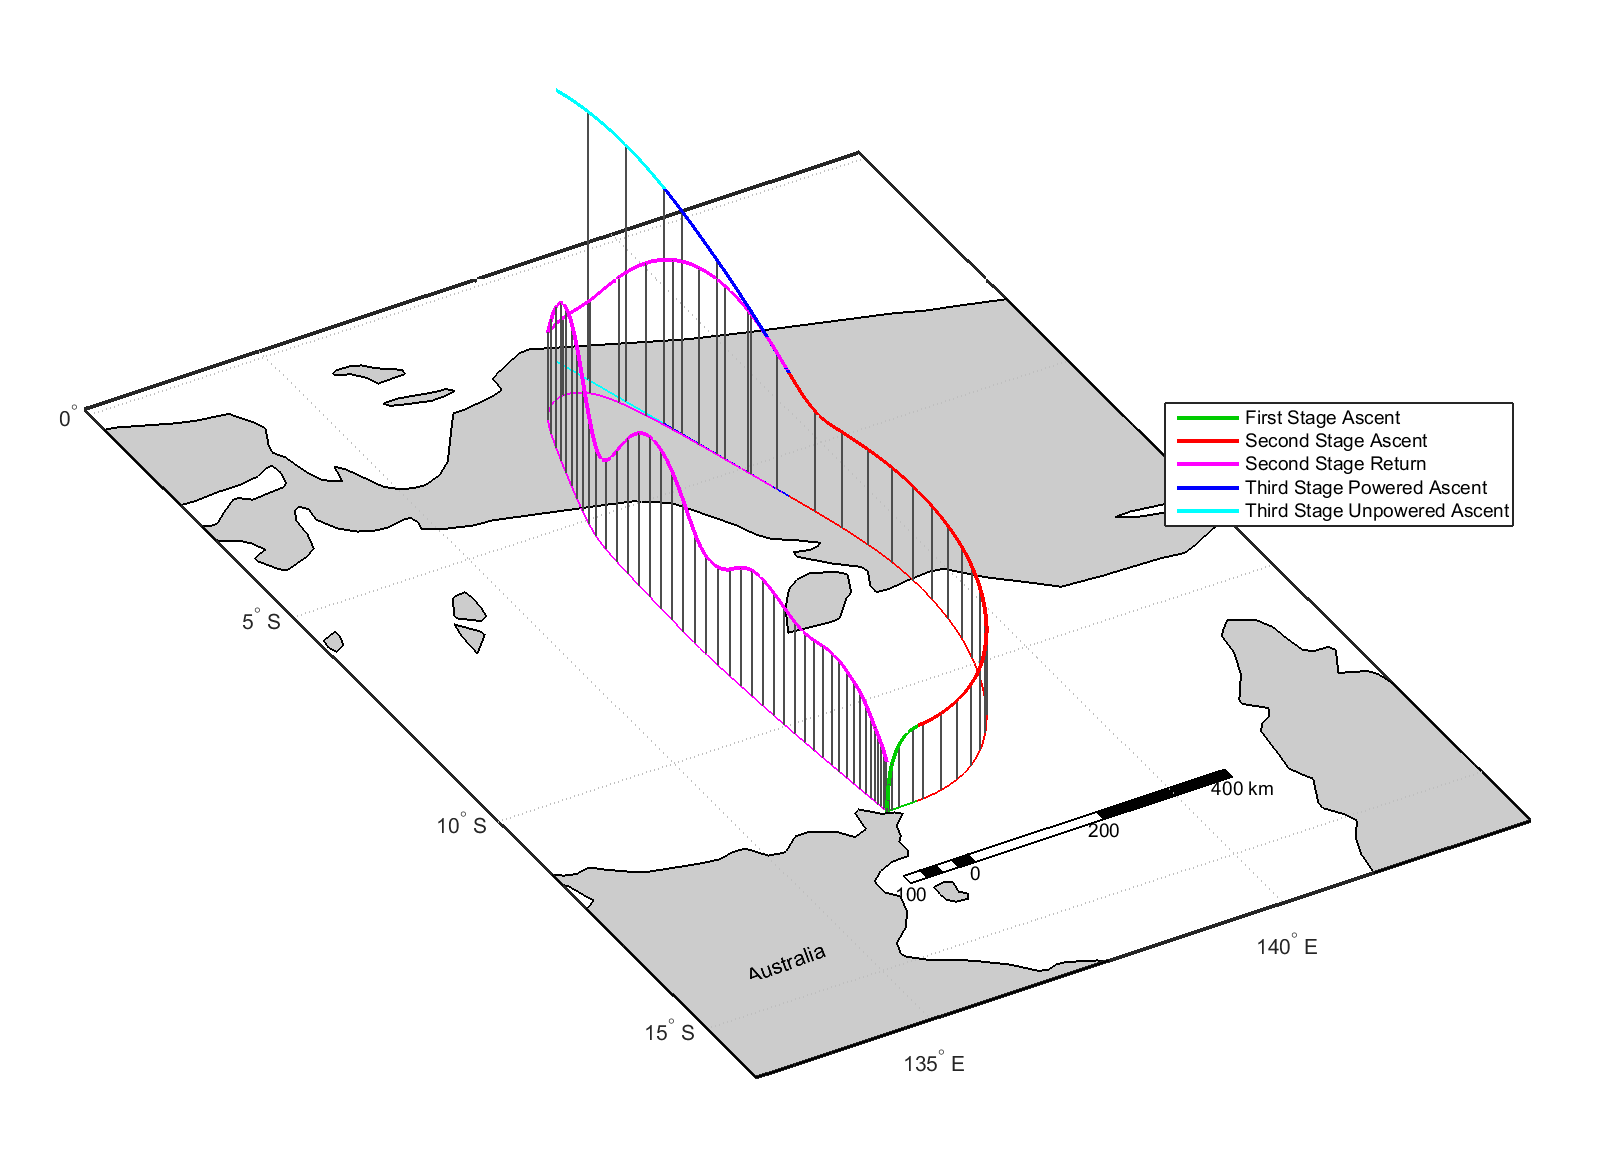
\includegraphics[width=1\linewidth]{../LODESTAR_FINAL/Results/mode11/GroundTrackStandard}
	\caption{Maximum payload-to-orbit trajectory path with the inclusion of SPARTAN fly-back (Case 11). Initial heading angle of -12.44$^\circ$.}
	\label{fig:GroundTrackStandard}
\end{figure}
The maximum payload-to-orbit is reduced by -10.0\% compared to the optimised trajectory result without fly-back. The benefits of flying back the SPARTAN to its initial launch site, compared to the alternative of transporting the SPARTAN back to the launch site from a remote landing, are likely to far outweigh this associated reduction in payload. 



\section{Ascent Trajectory}

 After launch, the first stage pitches towards the east, beginning at a heading angle of -12.4$^\circ$.
 Other than this heading angle difference, the first stage trajectory, shown in Figure \ref{fig:FirstStageStandard}, is very similar to that of the first stage launching the SPARTAN with no return flight, detailed in Section \ref{sec:optimisednoreturn}, with the exception of a small adjustment manoeuvre. 
 After pitchover, the first stage gradually reduces the angle of attack to a minimum of -0.47$^\circ$ at 30.9s flight time, in order to make small adjustments to the pitch profile while the velocity is low. After this, the first stage angle of attack returns to 0$^\circ$ at 42.9s flight time, and is maintained for 16.4s.
 The angle of attack is then reduced, to a minimum of -3.58$^\circ$ in order to adjust the altitude and trajectory angle, before increasing back to 0$^\circ$ at first stage-SPARTAN separation. 
 The SPARTAN is released in an easterly direction, at a heading angle of -12.4$^\circ$, an altitude of \firstsecondSeparationAltStandard km, and a trajectory angle of \firstsecondSeparationgammaStandard $^\circ$. 
 This altitude of first stage-SPARTAN separation is 3.02km (+12.5\%) higher than the first stage-SPARTAN separation point with no fly-back, with a trajectory angle at separation which is +2.5$^\circ$ (+80.6\%) higher. 
 This higher release point increases the exergy efficiency of the first stage rocket by +0.308\%$\eta$ (+4.9\%), and allows the first stage to achieve a higher velocity at separation (an increase of +64m/s, +4.3\%). 
 
 The higher altitude, larger trajectory angle, and increased velocity at the first stage-SPARTAN separation point causes an altitude raising manoeuvre at the beginning of the SPARTAN's acceleration, which is significantly higher than the altitude raising manoeuvre with no fly-back. This altitude raising manoeuvre takes the SPARTAN to a height of 29.59km at 31.44s, and decreases the dynamic pressure of the SPARTAN to 29.1kPa, allowing time for the bank angle of the SPARTAN to be increased. 
 The SPARTAN performs a banking turn during the entirety of its acceleration. After the first stage-SPARTAN separation, the bank angle is increased, at the maximum change rate, to 44.2$^\circ$, which aids the SPARTAN in decreasing its altitude. As the altitude of the SPARTAN begins to reduce, the bank angle stops increasing and the angle of attack is increased to 3.24$^\circ$, to increase the lift, slowing the descent of the SPARTAN. 
 The bank angle then begins to increase once more, and as the SPARTAN reaches close to its maximum dynamic pressure at 109.8s, the angle of attack is reduced, and the bank angle reaches an initial maximum of 56.8$^\circ$. 
\begin{figure}[ht!]
\centering
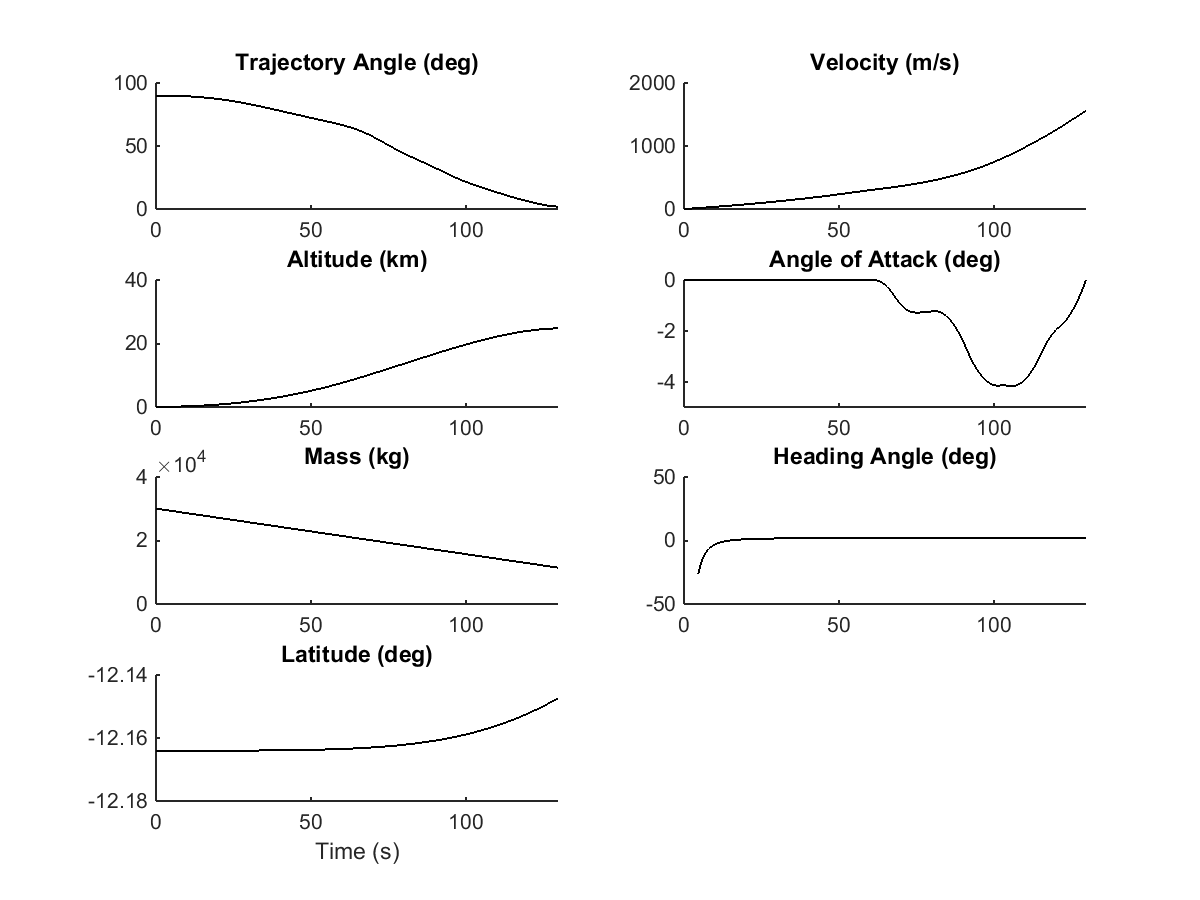
\includegraphics[width=0.7\linewidth]{../LODESTAR_FINAL/Results/mode11/FirstStageStandard}
\caption{The first stage of the optimised maximum payload-to-orbit trajectory with SPARTAN fly-back (Case 11). }
\label{fig:FirstStageStandard}
\end{figure}
\begin{figure}[ht!]
\centering
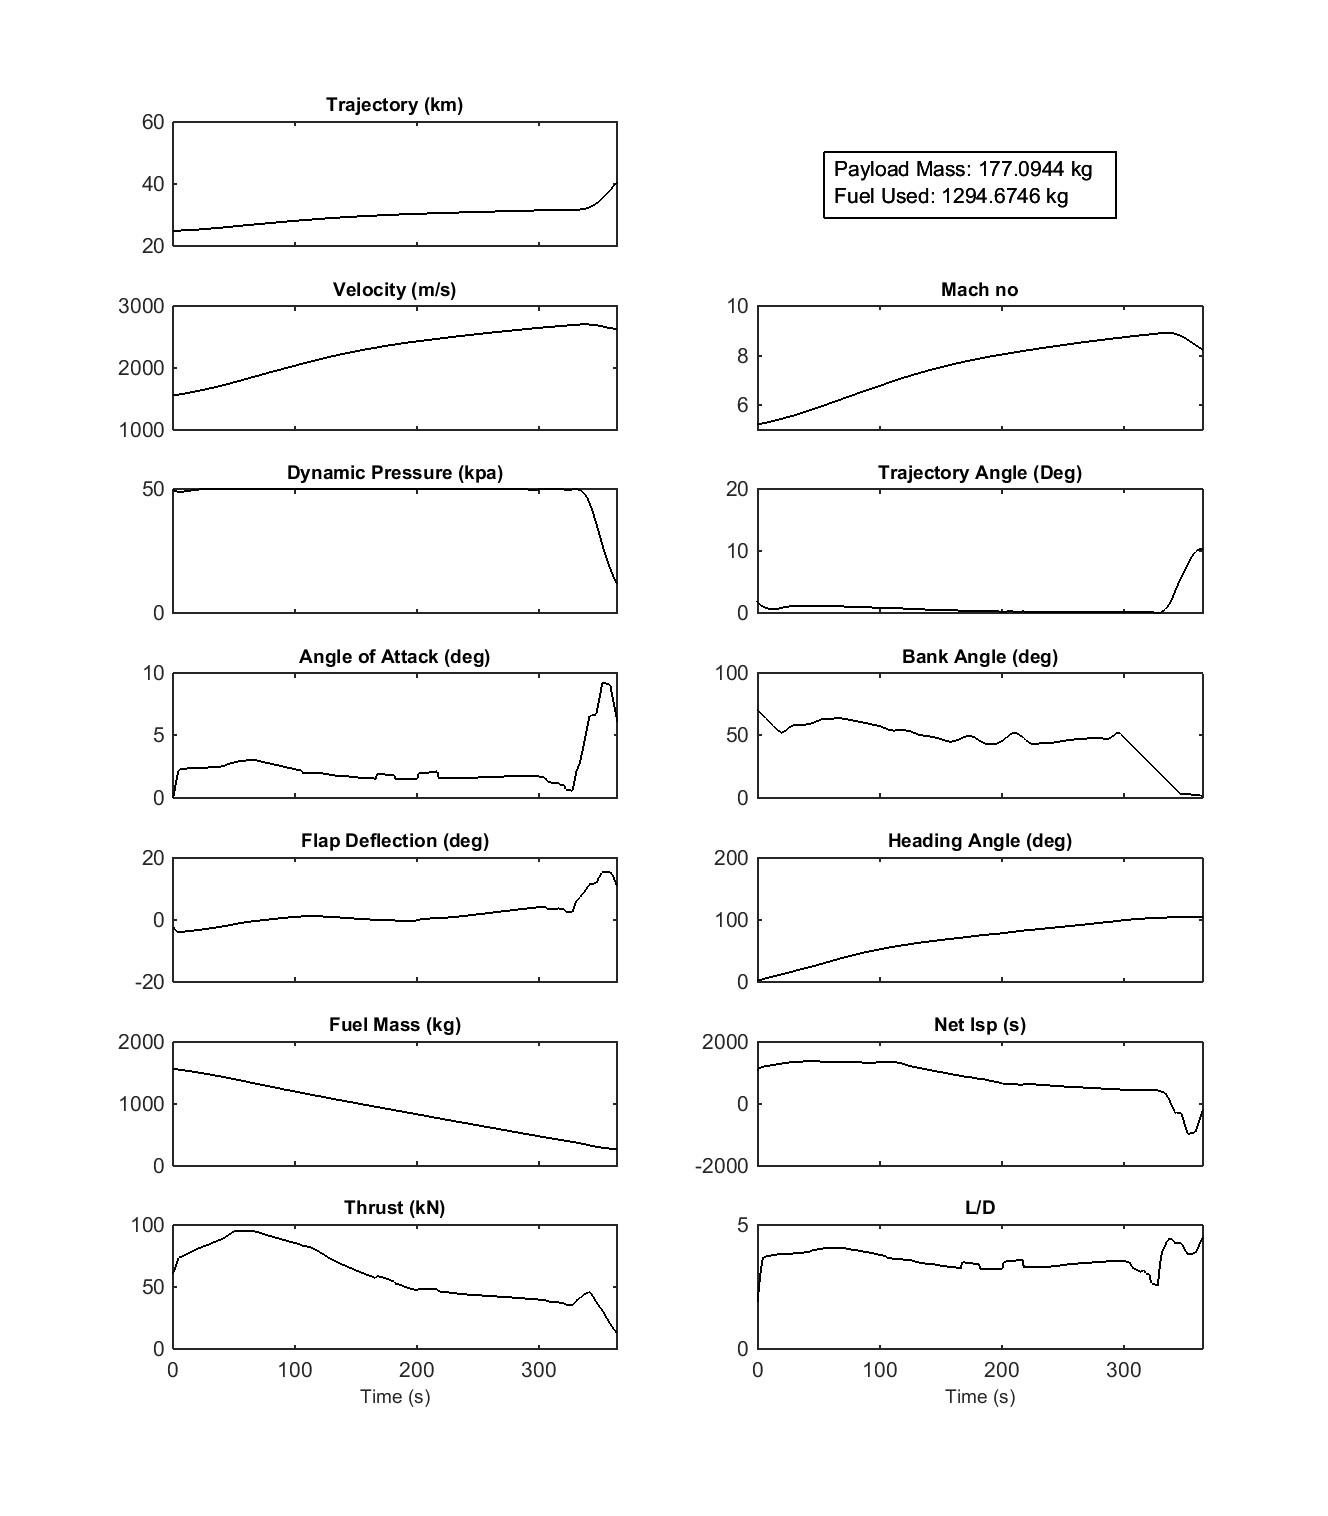
\includegraphics[width=1\linewidth]{../LODESTAR_FINAL/Results/mode11/SecondStageStandard}
\caption{The acceleration of the SPARTAN flying an optimised maximum payload-to-orbit trajectory with SPARTAN fly-back (Case 11). }
\label{fig:SecondStageStandard}
\end{figure}
\begin{figure}[ht!]
\centering
\includegraphics[width=0.9\linewidth]{../LODESTAR_FINAL/Results/mode11/NetIspStandard}
\caption{Net $I_{SP}$ contours for the SPARTAN at Mach numbers between 6 and 8, showing the optimised trajectory path. }
\label{fig:NetIspStandard}
\end{figure}
The bank angle of the SPARTAN is then reduced, and afterwards is maintained between 50.4$^\circ$ and 58.6$^\circ$, exhibiting higher bank angles towards the latter part of the ascent. At the end of the SPARTAN's acceleration, the bank angle is reduced, so that the third stage is released at 0$^\circ$ bank angle. This 0$^\circ$ bank angle is defined as a constraint on the end of the trajectory, to ensure that the third stage rocket is released in the vertical plane, and is able to manoeuvre to orbit. 

The angle of attack of the SPARTAN is significantly higher over the course of the maximum payload-to-orbit trajectory with fly-back inclusion, compared to maximum payload-to-orbit trajectory with no fly-back, detailed in Section \ref{sec:optimisednoreturn}. These significantly  higher angles of attack are a result of the high bank angle of the SPARTAN throughout its trajectory, which cause the lift of the SPARTAN to be partially used for changing the heading of the SPARTAN, rather than providing vertical force. 
 The higher angles of attack result in the optimal trajectory of the SPARTAN following a close to maximum dynamic pressure path for most of the duration of its trajectory, without the altitude raising manoeuvre observed in Section \ref{sec:optimisednoreturn}.
 The increase in angle of attack means that the SPARTAN no longer flies within the homogeneous region of the specific impulse of the C-REST engines. instead the flight conditions are close to a region where an increase in angle of attack causes a sharp decrease in specific impulse. 
This indicates that at Mach 7 and 8, the angle of attack, and consequently the allowable bank angle, of the SPARTAN is being limited by the performance of the C-REST engines. 
 The SPARTAN stays close to its maximum dynamic pressure until a pull-up is performed at 365.8s flight time. 

The higher angles of attack flown by the SPARTAN also have the consequence of decreasing the net specific impulse of the SPARTAN during its acceleration, with the maximum specific impulse being decreased by -2.5\%.
The overall exergy efficiency of the SPARTAN is decreased, to \secondExergyEffStandard\%$\eta$, a decrease of -0.729\%$\eta$ (-15.4\%) compared to the maximum payload-to-orbit trajectory with no fly-back. This exergy efficiency decrease is due partially to the decrease in the specific impulse of the scramjet engines, but more significantly is attributed to the fuel necessary for the return flight resulting in less fuel being available for the ascent of the SPARTAN, and thus less `useful' work being attained from the total fuel mass.
A total fuel mass of 1294kg is used during the SPARTAN's acceleration, out of a total of 1562kg of available fuel. This reduction in fuel mass used, along with the reduction in net specific impulse due to the higher angle of attack values, reduces the velocity at SPARTAN-third stage separation by -106m/s (-3.9\%) compared to the maximum payload-to-orbit case with no SPARTAN fly-back. The SPARTAN pulls up to \secondthirdSeparationAltStandard km altitude and \secondthirdSeparationgammaStandard $^\circ$ before SPARTAN-third stage separation, a difference of only -0.8km (-1.9\%) and +0.2$^\circ$ (+1.8\%) compared to the maximum payload-to-orbit trajectory without fly-back, indicating that the inclusion of fly-back does not have a large effect on the magnitude of the pull-up manoeuvre. 

The exergy efficiency of the third stage is decreased by -1.845\%$\eta$ (-9.8\%) when compared to the maximum payload-to-orbit trajectory with no SPARTAN fly-back, due to the lower velocity of the third stage release increasing the losses of the third stage due to propulsive inefficiencies. 


\begin{figure}[ht!]
\centering
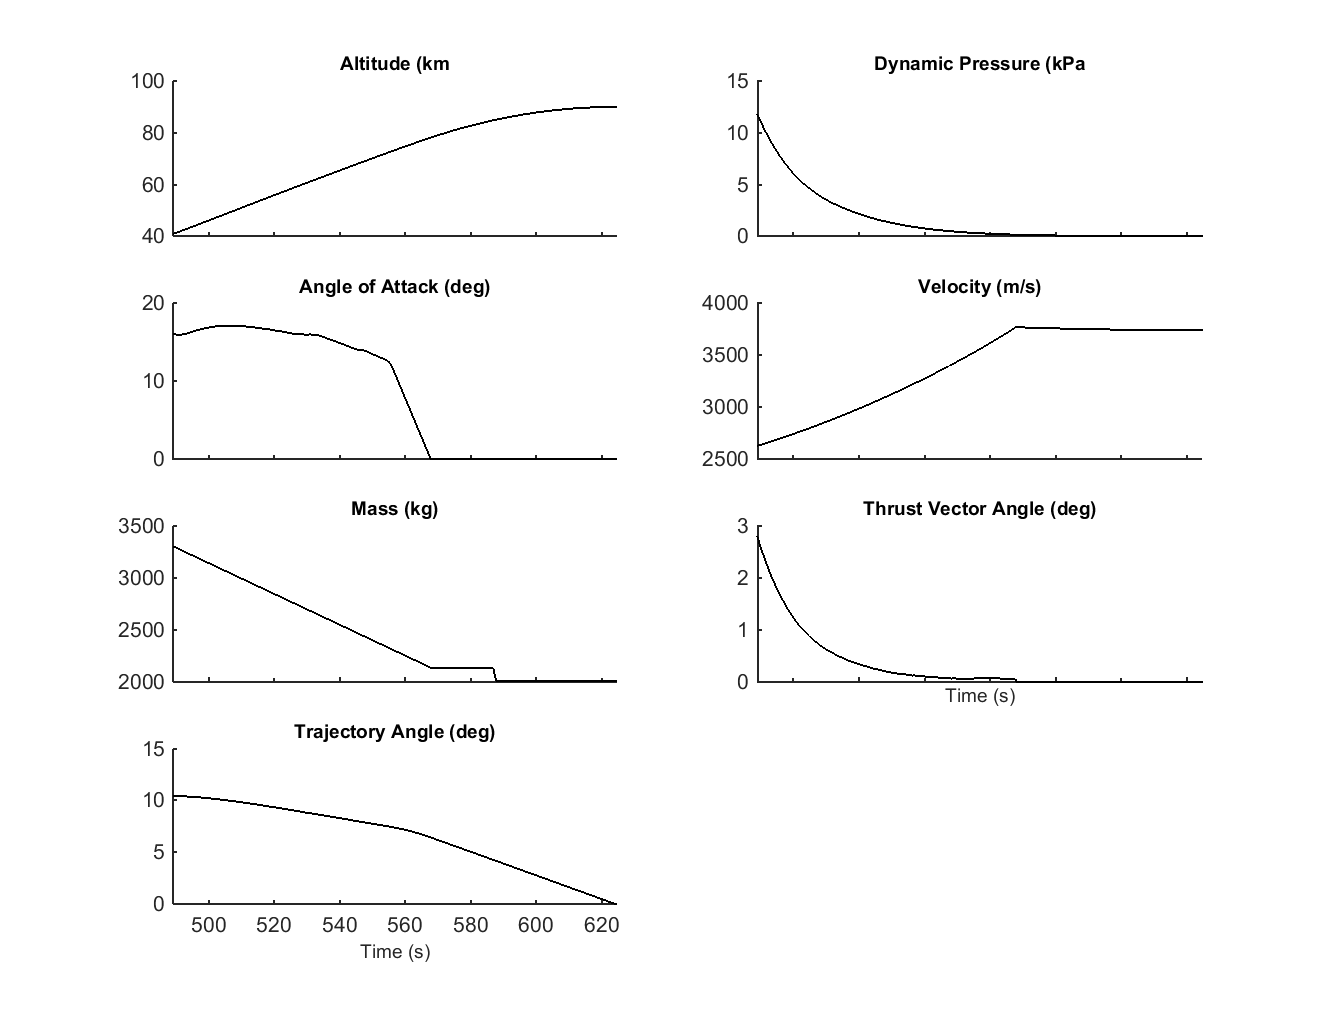
\includegraphics[width=1\linewidth]{../LODESTAR_FINAL/Results/mode11/ThirdStageStandard}
\caption{The third stage trajectory of an optimised maximum payload-to-orbit trajectory with SPARTAN fly-back (Case 11). }
\label{fig:ThirdStageStandard}
\end{figure}


\section{Fly-Back Trajectory}

\begin{figure}[ht!]
	\centering
	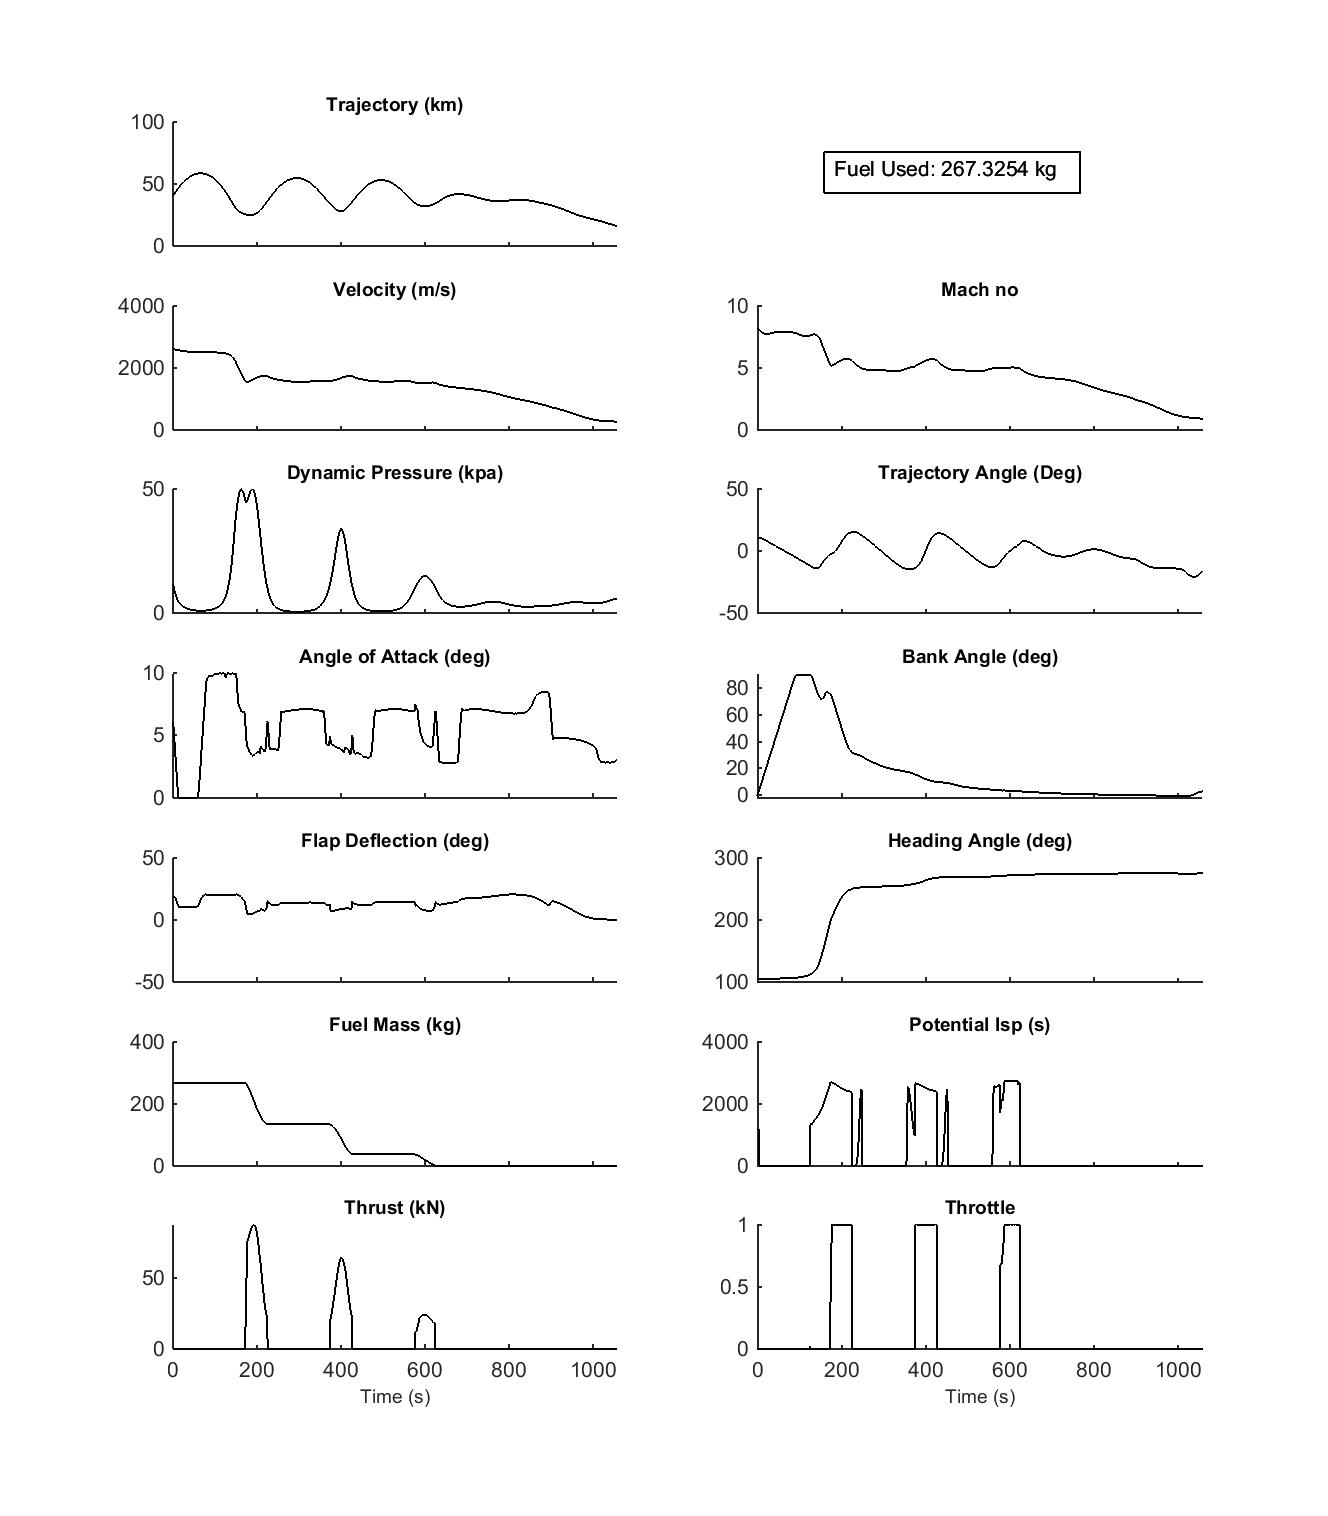
\includegraphics[width=1\linewidth]{../LODESTAR_FINAL/Results/mode11/ReturnStandard}
	\caption{The fly-back trajectory of the SPARTAN flying an optimised maximum payload-to-orbit trajectory (Case 11). }
	\label{fig:ReturnStandard}
\end{figure}

The optimised fly-back trajectory is shown in Figure \ref{fig:ReturnStandard}.
The SPARTAN is shown to be capable of fly-back, using \returnFuelStandard kg of fuel, 17.2\% of the total fuel.
Throughout its fly-back the SPARTAN performs distinct skipping manoeuvres, and ignites the scramjet engines a total of three times. 
The skips are aided by the angle of attack of the SPARTAN, and are consistent with previous research which has shown that a periodic skipping trajectory increases the downrange distance achievable by hypersonic vehicles both during powered and unpowered flight\cite{Eggers1957,Kanda2007}. These skips serve to reduce the fuel necessary for the return flight. 

It is observed that the optimised trajectory exhibits characteristics which can be separated into three distinct segments; 1. initial turn, 2. boost-skip phase, and 3. approach, as indicated in Figure \ref{fig:ReturnStandard}. 
 
\subsubsection{ Initial Turn}
The SPARTAN separates from the third stage rocket at a bank angle of 0$^\circ$, and then increases its bank angle at close to the maximum change rate until 108.7s return flight time, at which point 81.7$^\circ$ bank angle is reached. This high bank angle serves to rapidly change the heading of the SPARTAN, in order to minimise the down-range distance flown, and reduce the fuel necessary for fly-back. 
The angle of attack is kept low during this time, in order to minimise the size of the initial skip. 
As the SPARTAN reaches the zenith of its initial skip, at 66.1s flight time and 60.0km altitude, the angle of attack is rapidly increased, up to a maximum of 8.76$^\circ$. 
This increase in angle of attack, along with the aid of a subsequent reduction in the bank angle to 67.5$^\circ$, generates additional lift to slow the descent of the SPARTAN into the trough of the first skip, ensuring that the dynamic pressure limit is not exceeded. 


\subsubsection{ Boost-Skip Phase}\label{sec:boost}
At 182.8s flight time, the scramjet engines are ignited. The C-REST engines are powered-on in the trough between the first and second skips, at a point of high potential specific impulse, and initially burn for 22s. During the initial burn, the lift/drag of the SPARTAN increases significantly, due to the scramjet engine flow paths of the SPARTAN generating thrust, rather than drag. 
This increase in L/D raises the altitude of the SPARTAN and, along with the bank angle of 62.2$^\circ$, changes the heading of the SPARTAN significantly. 
The burn is limited by the lower inlet dynamic pressure limit of the C-REST engines, of 20kPa, and terminates at 204.8s flight time. After the initial burn ends, the angle of attack of the SPARTAN is decreased to 3.2$^\circ$, and the SPARTAN executes its second skip. Once the SPARTAN is descending again, and as soon as the dynamic pressure is high enough for C-REST engine operation at 339.9s return flight time, the scramjet engines are once again ignited.
During the second burn, the angle of attack of the SPARTAN is increased, to modify the temperature and Mach number at the inlet of the C-REST engines so that the maximum specific impulse is obtained from the C-REST engines during the burn. 
The angle of attack varies between 4.2$^\circ$ to 3.3$^\circ$ during the second burn, and the lift/drag is once again raised significantly, initiating the third skip. 
This skip raises the altitude of the SPARTAN to 54.6km, before it decreases once again. 
The third and last burn is initiated at 536.7s and lasts until 579.0s, when the remaining fuel has been depleted. Before the third burn, the angle of attack is decreased, so that it varies between 4.5$^\circ$ and 3.7$^\circ$ during the burn. These angle of attack values are similar to those observed during the second burn, indicating that these angle of attack values obtain a high specific impulse from the C-REST engines, this can be observed in Figure \ref{fig:returnIspStandard}, which shows the specific impulse profile of the return flight during the boost-skip phase. 

After the third burn phase, the angle of attack is initially controlled so that the skipping trajectory of the SPARTAN is dampened.
Immediately after the third burn phase, the angle of attack is reduced, to 2.82$^\circ$. This reduction coincides with the ascent portion of the fourth skip, reducing the lift, and the amount of altitude gained. 
As the zenith of the forth skip is reached, the angle of attack is increased to 7.2$^\circ$, increasing the lift, and once again slowing the descent. 
This high angle of attack is sustained until 748.2s at which point the angle of attack is reduced again significantly, to 2.6$^\circ$, reducing the size of the fifth skip. At 871.2s, the angle of attack is again raised, to 5$^\circ$, initiating the sixth and last skip.
It is notable that the sixth skip is initiated in this way, as previously in the unpowered portion of the trajectory the angle of attack is being utilised to damped the skipping motion. This indicates that some degree of skipping is desirable after the final scramjet burn, and that the angle of attack is being controlled to produce optimally sized skips. 

\subsubsection{ Approach}

After the final small skip, at 993.3s flight time, the angle of attack is adjusted, so that a gradual, controlled descent is initiated. 
After the skip phase, as the vehicle is approaching Mach 1, the angle of attack is reduced gradually to bring the SPARTAN down to 1km altitude, in a controlled manner. At 1227.0s, the bank angle is increased, in order to perform a final adjustment of the heading angle, to bring the SPARTAN to the desired end location. 
The SPARTAN reaches 1km altitude at -26.7$^\circ$ trajectory angle and 120.0m/s velocity (Mach 0.356). It is assumed that the SPARTAN is able to perform a landing manoeuvre after this point. 





\section{Energy Usage Analysis}


\begin{table}[ht]
	\centering
	\begin{tabular}{l c c} 
		\hline \textbf{Trajectory Condition}
		& No Fly-Back
		& With Fly-Back
		\\
		\textbf{First Stage Fuel Exergy} 
		&\textbf{\firstEnergyStandardNoReturn} GJ
		&\textbf{\firstEnergyStandard} GJ
		\\
		
		\textcolor{blue}{KE + PE of Payload}
		& \firstWpayloadStandardNoReturn \% (0.25 GJ)
		& \firstWpayloadStandard \% (0.25 GJ)
		\\
		\textcolor{red}{KE + PE of  2$^{nd}$ \& 3$^{rd}$ Stage}
		& \firstWnextStageStandardNoReturn \% (12.87 GJ) & \firstWnextStageStandard \% (14.12 GJ)
		\\
		\textcolor{red}{Overcoming Drag} 
		& \WDoneStandardNoReturn \% (3.44 GJ) & \WDoneStandard \% (2.92 GJ)
		\\
		\textcolor{red}{KE + PE of 1$^{st}$ Stage Structural Mass} 
		& \WoneStandardNoReturn \% (2.19 GJ) & \WoneStandard \% (2.39 GJ)
		\\
		
		
		\textcolor{red}{Propulsion Inefficiency} 
		& \PlossoneCombinedStandardNoReturn \% (189.78 GJ) & \PlossoneCombinedStandard \% (197.96 GJ)
		\\ 
		\textbf{SPARTAN Fuel Exergy} 
		& \textbf{\secondEnergyStandardNoReturn} GJ & \textbf{\secondEnergyStandard} GJ
		\\
		\textcolor{blue}{KE + PE of Payload}
		& \secondWpayloadStandardNoReturn \% (0.51 GJ) & \secondWpayloadStandard \% (0.38J)
		\\
		\textcolor{red}{KE + PE of 3$^{rd}$ Stage}
		& \secondWnextStageStandardNoReturn \% (8.33 GJ) & \secondWnextStageStandard \% (7.09 GJ)
		\\
		\textcolor{red}{Overcoming Drag}
		& \WDsecondStandardNoReturn \% (36.76 GJ) & \WDsecondStandard \% (31.56 GJ)
		\\
		\textcolor{red}{KE + PE of SPARTAN Structural Mass}  
		& \WsecondStandardNoReturn \% (13.28 GJ) & \WsecondStandard \% (11.22 GJ)
		\\
		\textcolor{red}{Propulsion Inefficiency}  
		& \PlosssecondCombinedStandardNoReturn \% (128.51 GJ) & \PlosssecondCombinedStandard \% (104.97 GJ)
		\\
		
		
		
		\textbf{Return Fuel Exergy} 
		& - & \textbf{\returnEnergyStandard} GJ
		\\
		KE + PE of SPARTAN Structural Mass
		& - & \WreturnStandard \% (18.40 GJ)
		\\
		\textcolor{red}{Overcoming Drag}
		& - & \WDreturnStandard \% (30.94 GJ)
		\\
		
		\textcolor{red}{Propulsion Inefficiency}  
		& - & \PlossreturnCombinedStandard \% (19.61 GJ)
		\\
		
		
		\textbf{Third Stage Fuel Exergy}  
		& \textbf{\thirdEnergyStandardNoReturn} GJ & \textbf{\thirdEnergyStandard} GJ
		\\
		\textcolor{blue}{KE + PE of Payload}  
		&\thirddExergyEffStandardNoReturn \% (6.42 GJ) &\thirddExergyEffStandard \% (5.83 GJ)
		\\
		\textcolor{red}{Overcoming Drag}  
		& \WDthreeStandardNoReturn \% (0.20 GJ) & \WDthreeStandard \% (0.22 GJ)
		\\
		\textcolor{red}{KE + PE  of 3$^{rd}$ Stage Structural Mass}  
		& \WthreeStandardNoReturn \% (9.56 GJ) & \WthreeStandard \% (9.63 GJ)
		\\
		
		
		
		\textcolor{red}{KE + PE of Heat Shield}  
		
		& \WHSthreeStandardNoReturn \% (1.02 GJ) & \WHSthreeStandard \% (1.04 GJ)
		\\
		
		\textcolor{red}{Propulsion Inefficiency}  
		& \PlossthreeCombinedStandardNoReturn \% (17.09 GJ) & \PlossthreeCombinedStandard \% (17.80 GJ)
		\\
		\hline 
	\end{tabular} 
	\caption{An energy usage breakdown of the ascent trajectories, both with, and without, SPARTAN fly-back (Cases 11 \& 2). Blue indicates a 'productive' energy usage, whereas red indicates energy 'wastage'. Negative energy indicates energy being supplied.}
	\label{tab:effStandard}
\end{table}


An energy usage analysis is conducted for a maximum payload-to-orbit trajectory, including the fly-back of the SPARTAN. This is compared to the energy usage breakdown of the optimised trajectory without fly-back of the SPARTAN in Table \ref{tab:effStandard}. Similarly to Section \ref{sec:exergy1}, the energy used to accelerate the payload is shown, along with the energy imparted to the successive stages; the energy used overcoming drag; the energy used imparting energy to the structural mass of each stage, which is separated; and the energy lost due to propulsion inefficiency. 



The first stage rocket starts with a larger fuel mass when the fly-back of the SPARTAN is included, and thus starts with a larger fuel exergy. Overall, when the fly-back is included, more of the exergy of the first stage is utilised imparting energy upon the combination of the payload and the successive stages, at 6.6\% (14.37GJ), compared to 6.292\% ( 13.12GJ) without SPARTAN fly-back. This is due to the rocket flying a more efficient trajectory, with lower drag and propulsive losses, terminating at a higher altitude and velocity.

 
When flying a trajectory where the SPARTAN's fly-back is included, the drag losses during the ascent of the SPARTAN consist of a larger percentage of the fuel exergy usage  (\WDsecondStandard \%, compared to \WDsecondStandardNoReturn \% without fly-back). These increased drag losses are due to the less favourable first stage-SPARTAN separation conditions, and the high banking throughout the acceleration. However, the percentage of energy loss due to propulsive inefficiency is lower when fly-back is included, at \PlosssecondCombinedStandard \%, compared to \PlosssecondCombinedStandardNoReturn \% without fly-back. This is due to the lower total acceleration of the SPARTAN when fly-back is included, which results in flight over a more efficient propulsion regime. 
Overall, when the fly-back is included, the SPARTAN imparts a larger percentage of its available energy to the payload and third stage, at 5.196\%, compared to 4.718\% without fly-back.
However, the fly-back of the SPARTAN reduces the fuel, and thus the fuel exergy, available to the SPARTAN during ascent, causing less total energy to be imparted to the payload and third stage (7.47GJ), compared to the trajectory without fly-back (8.84GJ). 
This results in the third stage separating at a lower velocity, and at a lower altitude. This lower, slower separation point, when fly-back is included, causes the losses of the third stage to increase from all sources. The propulsive inefficiency losses are particularly affected, increasing from \PlossthreeCombinedStandard \% (17.80 GJ) without fly-back to \PlossthreeCombinedStandardNoReturn \% (17.09 GJ) with fly-back, due to the lower velocity of the separation point, which decreases the propulsive efficiency of the third stage (illustrated by Equation \ref{eq:rocketeff}).

The energy necessary to return the SPARTAN to its initial launch location is provided by both the fuel used during the return (32.15GJ), as well as the kinetic and potential energy imparted upon the SPARTAN during its ascent (18.40GJ). Significantly more energy is required to overcome drag during the return (30.94GJ) than is available from the kinetic and potential energy of the SPARTAN (18.40 GJ), illustrating the necessity for igniting the scramjet engines during the return flight. 





\section{Design Sensitivity Analysis}\label{sec:sensitivity}

It has been shown that the fly-back of the SPARTAN accelerator has a significant effect on the performance of the rocket-scramjet-rocket launch system, and that the maximum payload-to-orbit optimised trajectory changes significantly to compensate for the additional requirement of successfully returning the SPARTAN stage. This section investigates the sensitivity of the launch system to changes in the vehicle design, with the fly-back of the SPARTAN included. This sensitivity study varies the following:
\begin{itemize}
	\item Case 12: Dynamic Pressure, 
	\item Case 13: Specific Impulse,
	\item Case 14: SPARTAN Drag,
	\item Case 15: SPARTAN Mass,
	\item Case 16: SPARTAN Fuel Mass,
	\item Case 17: Third Stage Mass,
	\item Case 18: Third Stage Thrust.
\end{itemize}
As in Section \ref{sec:sensitivityNoReturn}, the effect of third stage drag is negligible. For this reason, variation in the third stage drag is omitted from this study. 

The launch system is able to successfully place a small satellite in orbit for every varied performance condition which has been tested, while returning the SPARTAN to its initial launch location for landing. 
Every maximum payload-to-orbit optimised trajectory exhibits considerable banking during the SPARTAN's ascent trajectory, as well as a pull-up of the SPARTAN before third stage release. 
In every case the optimised return flight path exhibits an initial turn, boost and approach phase, with multiple skipping manoeuvres. 
However, two aspects of the optimised trajectories vary between cases, exhibiting no clear trend across the sensitivity studies which have been performed; the first stage-SPARTAN release conditions; and the height, and duration, of the second skip of the return phase. 

The first stage-SPARTAN separation angle and altitude shows no clear trend in any of the sensitivity studies performed, except for the third stage mass variation, in contrast to the sensitivity study with no fly-back, detailed in Section \ref{sec:sensitivityNoReturn}, in which the SPARTAN mass and drag parameters change the first stage separation point significantly. All of the optimised trajectory solutions show a distinct initial altitude raising manoeuvre performed by the SPARTAN, however, the size is inconsistent across optimised trajectory solutions, indicating that this manoeuvre is no longer solely a product of an efficiency trade-off between the first stage pitching and SPARTAN engine efficiency.
In the maximum payload-to-orbit optimised trajectories calculated during the sensitivity analysis, it is observed that the trajectory angle at first-second stage release varies significantly between the optimised trajectories, with no discernible trend. When the SPARTAN is released at a high trajectory angle, it spends a significant amount of time in a low dynamic pressure environment, giving time for the bank angle to increase. The high bank angle is utilised during the descent of the SPARTAN onto the maximum dynamic pressure path, to rapidly change the heading of the SPARTAN. 
 A lower release angle results in the SPARTAN banking more, and flying a slightly less efficient trajectory. However, a lower release angle also results in the SPARTAN using its fuel more rapidly, and covering less ground, which results in the fly-back requiring less fuel. 
The trade-off between first stage efficiency and the initial operational efficiency of the SPARTAN appears to be close, and 
for each particular trajectory optimisation one or the other is favoured with no clear trend. 


It is also observed that there are two distinct return trajectory shapes for the return trajectory of the SPARTAN. The more common return trajectory shape has been shown in the preceding section, and consists of three or more large skips to begin the return trajectory. The second trajectory shape exhibits a small second skip, with the first two burns very closely spaced, or combined into one longer burn. An example of this second type of return trajectory is shown in Figure \ref{fig:ReturnComparison10}. During the first two burns, a higher bank angle is maintained when compared to the large skip trajectory shape, however, after the first two burns are completed, the bank angle is reduced more rapidly. 
During simulations, it was observed that on occasion, the optimal return trajectory type would change as the initial guess or problem setup was altered, with no significant change in the payload-to-orbit capabilities of the launch system. This variability suggests that there is minimal difference between the two shapes of return trajectory, and that both can potentially lead to efficient return flights. 





\subsection{Case 12: Dynamic Pressure Variation with Fly-Back Inclusion}

\begin{table}[ht]
	\centering
	\begin{tabular}{l c c c c c c} 
		\hline \textbf{Trajectory Condition}   \qquad  $q_{max}$:
		&40kPa
		&45kPa
		&50kPa
		&55kPa
		&60kPa
		& $\Delta/\Delta$/\%$q_{max}$
		\\
		\hline \textbf{Payload to Orbit (kg)}
		& \textbf{\PayloadToOrbitqForty}
		& \textbf{\PayloadToOrbitqFortyFive}
		& \textbf{\PayloadToOrbitqStandard}
		& \textbf{\PayloadToOrbitqFiftyFive}
		& \textbf{\PayloadToOrbitqSixty}
		&\textbf{0.4}
		\\
		\textbf{Payload Variation (\%)}
		& \PayloadVarqForty
		& \PayloadVarqFortyFive
		& \PayloadVarqStandard
		& \PayloadVarqFiftyFive
		& \PayloadVarqSixty
		&0.25
		\\
		\textbf{Total $\eta_{exergy}$ (\%)}
		& \textbf{\totalExergyEffqForty}
		& \textbf{\totalExergyEffqFortyFive}
		& \textbf{\totalExergyEffqStandard}
		& \textbf{\totalExergyEffqFiftyFive}
		& \textbf{\totalExergyEffqSixty}
		& \textbf{3e-05}
		\\
		\hline 
		\textbf{1$^{st}$ Stage $\eta_{exergy}$ (\%)}
		& \textbf{\firstExergyEffqForty}
		& \textbf{\firstExergyEffqFortyFive}
		& \textbf{\firstExergyEffqStandard}
		& \textbf{\firstExergyEffqFiftyFive}
		& \textbf{\firstExergyEffqSixty}
		& -
		\\
		\textbf{Separation Alt, 1$\rightarrow$2 (km)}
		& \firstsecondSeparationAltqForty
		& \firstsecondSeparationAltqFortyFive
		& \firstsecondSeparationAltqStandard
		& \firstsecondSeparationAltqFiftyFive
		& \firstsecondSeparationAltqSixty
		& -
		\\
		\textbf{Separation v, 1$\rightarrow$2 (m/s)}
		& \firstsecondSeparationvqForty
		& \firstsecondSeparationvqFortyFive
		& \firstsecondSeparationvqStandard
		& \firstsecondSeparationvqFiftyFive
		& \firstsecondSeparationvqSixty
		& -
		\\
		\textbf{Separation $\gamma$, 1$\rightarrow$2 (deg)}
		& \firstsecondSeparationgammaqForty
		& \firstsecondSeparationgammaqFortyFive
		& \firstsecondSeparationgammaqStandard
		& \firstsecondSeparationgammaqFiftyFive
		& \firstsecondSeparationgammaqSixty
		& -
		\\
		\hline 
		\textbf{2$^{nd}$ Stage $\eta_{exergy}$ (\%)}
		& \textbf{\secondExergyEffqForty}
		& \textbf{\secondExergyEffqFortyFive}
		& \textbf{\secondExergyEffqStandard}
		& \textbf{\secondExergyEffqFiftyFive}
		& \textbf{\secondExergyEffqSixty}
		& -
		\\
		\textbf{Separation Alt, 2$\rightarrow$3 (km)}
		& \secondthirdSeparationAltqForty
		& \secondthirdSeparationAltqFortyFive
		& \secondthirdSeparationAltqStandard
		& \secondthirdSeparationAltqFiftyFive
		& \secondthirdSeparationAltqSixty
		&-0.02
		\\
		\textbf{Separation $v$, 2$\rightarrow$3 (m/s)}
		& \secondthirdSeparationvqForty
		& \secondthirdSeparationvqFortyFive
		& \secondthirdSeparationvqStandard
		& \secondthirdSeparationvqFiftyFive
		& \secondthirdSeparationvqSixty
		&1.99
		\\
		\textbf{Separation $\gamma$, 2$\rightarrow$3 (deg)}
		& \secondthirdSeparationgammaqForty
		& \secondthirdSeparationgammaqFortyFive
		& \secondthirdSeparationgammaqStandard
		& \secondthirdSeparationgammaqFiftyFive
		& \secondthirdSeparationgammaqSixty
		& -
		\\
		\textbf{2$^{nd}$ Stage Flight Time (s)}
		& \secondFlightTimeqForty
		& \secondFlightTimeqFortyFive
		& \secondFlightTimeqStandard
		& \secondFlightTimeqFiftyFive
		& \secondFlightTimeqSixty
		&-1.58
		\\
		\textbf{2$^{nd}$ Stage Distance Flown (km)}
		& \SecondDistqForty
		& \SecondDistqFortyFive
		& \SecondDistqStandard
		& \SecondDistqFiftyFive
		& \SecondDistqSixty
		&-3.99
		\\
		\textbf{2$^{nd}$ Stage Return Fuel (kg)}
		& \returnFuelqForty
		& \returnFuelqFortyFive
		& \returnFuelqStandard
		& \returnFuelqFiftyFive
		& \returnFuelqSixty
		& -
		\\
		\textbf{2$^{nd}$ Stage Return Distance (km)}
		& \returnDistqForty
		& \returnDistqFortyFive
		& \returnDistqStandard
		& \returnDistqFiftyFive
		& \returnDistqSixty
		&-5.98
		\\
		\hline 
		\textbf{3$^{rd}$ Stage $\eta_{exergy}$ (\%)}
		& \textbf{\thirddExergyEffqForty}
		& \textbf{\thirddExergyEffqFortyFive}
		& \textbf{\thirddExergyEffqStandard}
		& \textbf{\thirddExergyEffqFiftyFive}
		& \textbf{\thirddExergyEffqSixty}
		& \textbf{0.042}
		\\
		\textbf{3$^{rd}$ Stage $t$, $q >$ 5kpa (s)}
		& \thirdqOverFiveqForty
		& \thirdqOverFiveqFortyFive
		& \thirdqOverFiveqStandard
		& \thirdqOverFiveqFiftyFive
		& \thirdqOverFiveqSixty
		& -
		\\
		\textbf{3$^{rd}$ Stage max $\alpha$ (deg)}
		& \thirdmaxAoAqForty
		& \thirdmaxAoAqFortyFive
		& \thirdmaxAoAqStandard
		& \thirdmaxAoAqFiftyFive
		& \thirdmaxAoAqSixty
		&0
		\\
		\textbf{3$^{rd}$ Stage Fuel Mass (kg)}
		& \thirdmFuelqForty
		& \thirdmFuelqFortyFive
		& \thirdmFuelqStandard
		& \thirdmFuelqFiftyFive
		& \thirdmFuelqSixty
		&-0.42
		\\
		\hline 
	\end{tabular} 
	\caption{Comparison of key trajectory parameters with variation in the maximum dynamic pressure of the SPARTAN, with fly-back (Case 12).}
	\label{tab:qvarreturn}
\end{table}


The maximum dynamic pressure allowable during flight is varied by $\pm$20\% in order to determine the sensitivity of the launch system to the structural and thermal limitations of the SPARTAN.  
Table \ref{tab:qvarreturn} shows a summary of the key parameters of each optimised trajectory, and trajectory comparison plots are shown in Appendix \ref{sec:app_comparison21}. The variation in each trajectory parameter per \% of the dynamic pressure is shown, if there is a clear trend. The payload-to-orbit of the launch system improves by +9.4kg (+5.51\%) at 60kPa, and decreases by -7.7kg (-4.52\%) at 40kPa.
The overall exergy efficiency of the system increases as the maximum dynamic pressure increases, by +0.083$\eta$\% at 60kPa, and decreases as the maximum dynamic pressure decreases, by -0.067$\eta$\% at 40kpa. 
No significant variation is observed between sensitivity studies with or without the fly-back included in the sensitivity of the launch system to the maximum dynamic pressure of the SPARTAN, by percentage.

When fly-back is included, no trends are observed in the exergy efficiencies of the first stage or SPARTAN, due to maximum dynamic pressure variation. Compared to the sensitivity study with no fly-back, the trade-offs between the efficiencies of the stages include the manoeuvrability of the SPARTAN, which dictates the fuel used during the return flight. This additional factor produces more complicated energy trade-offs, resulting in differing optimal trajectory shapes. This can particularly be observed in the 45kPa maximum dynamic pressure trajectory, which exhibits significantly different trade-offs between each stage, when compared to the other cases. 

 The 45kPa maximum dynamic pressure simulation shows a low exergy efficiency for the first stage than would be suggested by the general exergy efficiency trends. 
 However, the 45kPa simulation trades the performance of the first stage to achieve greater manoeuvrability at the beginning of the SPARTAN's trajectory, resulting in less fuel being used during fly-back, and a higher overall exergy efficiency for the SPARTAN. The first stage-SPARTAN separation occurs at a lower altitude and trajectory angle compared to the other simulations, allowing the acceleration to be achieved more quickly at the start of the trajectory, and enabling the SPARTAN to manoeuvre more effectively at the beginning of its trajectory. 
 As a consequence, the 45kPa simulation uses only 257.0kg of fuel during the fly-back, against the general trend of the return fuel usage. 

Excluding the 45kpa trajectory, increasing the maximum dynamic pressure improves the manoeuvring capabilities of the SPARTAN and increases the acceleration rate during ascent, which leads to a smaller flight time, and less ground coverage, reducing the amount of fuel necessary for fly-back. 
The exergy efficiency of the first stage is generally increased as the maximum dynamic pressure is increased, and the altitude at first stage-SPARTAN release is raised, again with the exception of the 45kpa case. 
The exergy efficiency of the SPARTAN is relatively consistent across the simulations, particularly when compared to the variance observed in the dynamic pressure sensitivity study with no fly-back, in Section \ref{sec:qvariation}.
This is due to the higher maximum dynamic pressure simulations using more fuel during the acceleration of the SPARTAN, and accelerating more over the trajectory (the velocity at SPARTAN-third stage separation increases by +51m/s, 2.0\%, at 60kpa maximum dynamic pressure, and decreases by -28m/s, 1.1\%, at 40kPa), resulting in the specific impulse of the scramjet engines being lower at the end of the acceleration. Overall, the SPARTAN is utilising more fuel mass at similar efficiencies, so that more overall `useful' work is being gained. 


\subsection{Case 13: SPARTAN Drag Sensitivity with Fly-Back Inclusion}


\begin{table}[ht]
	\centering
	\begin{tabular}{l c c c c c c} 
		\hline \textbf{Trajectory Condition}   \qquad  $C_{d,2}$:
		&90\%
		&95\%
		&100\%
		&105\%
		&110\%
		& $\Delta/\Delta$/\%$C_{d,2}$
		\\
		\hline \textbf{Payload to Orbit (kg)}
		& \textbf{\PayloadToOrbitCdNinety}
		& \textbf{\PayloadToOrbitCdNinetyFive}
		& \textbf{\PayloadToOrbitCdStandard}
		& \textbf{\PayloadToOrbitCdOneHundredFive}
		& \textbf{\PayloadToOrbitCdOneHundredTen}
		&\textbf{-1.5}
		\\
		\textbf{Payload Variation (\%)}
		& \PayloadVarCdNinety
		& \PayloadVarCdNinetyFive
		& \PayloadVarCdStandard
		& \PayloadVarCdOneHundredFive
		& \PayloadVarCdOneHundredTen
		&-0.9
		\\
		\textbf{Total $\eta_{exergy}$ (\%)}
		& \textbf{\totalExergyEffCdNinety}
		& \textbf{\totalExergyEffCdNinetyFive}
		& \textbf{\totalExergyEffCdStandard}
		& \textbf{\totalExergyEffCdOneHundredFive}
		& \textbf{\totalExergyEffCdOneHundredTen}
		& \textbf{-0.00013}
		\\
		\hline 
		\textbf{1$^{st}$ Stage $\eta_{exergy}$ (\%)}
		& \textbf{\firstExergyEffCdNinety}
		& \textbf{\firstExergyEffCdNinetyFive}
		& \textbf{\firstExergyEffCdStandard}
		& \textbf{\firstExergyEffCdOneHundredFive}
		& \textbf{\firstExergyEffCdOneHundredTen}
		& \textbf{-0.025}
		\\
		\textbf{Separation Alt, 1$\rightarrow$2 (km)}
		& \firstsecondSeparationAltCdNinety
		& \firstsecondSeparationAltCdNinetyFive
		& \firstsecondSeparationAltCdStandard
		& \firstsecondSeparationAltCdOneHundredFive
		& \firstsecondSeparationAltCdOneHundredTen
		& -
		\\
		\textbf{Separation v, 1$\rightarrow$2 (m/s)}
		& \firstsecondSeparationvCdNinety
		& \firstsecondSeparationvCdNinetyFive
		& \firstsecondSeparationvCdStandard
		& \firstsecondSeparationvCdOneHundredFive
		& \firstsecondSeparationvCdOneHundredTen
		&-3.66
		\\
		\textbf{Separation $\gamma$, 1$\rightarrow$2 (deg)}
		& \firstsecondSeparationgammaCdNinety
		& \firstsecondSeparationgammaCdNinetyFive
		& \firstsecondSeparationgammaCdStandard
		& \firstsecondSeparationgammaCdOneHundredFive
		& \firstsecondSeparationgammaCdOneHundredTen
		& -
		\\
		\hline 
		\textbf{2$^{nd}$ Stage $\eta_{exergy}$ (\%)}
		& \textbf{\secondExergyEffCdNinety}
		& \textbf{\secondExergyEffCdNinetyFive}
		& \textbf{\secondExergyEffCdStandard}
		& \textbf{\secondExergyEffCdOneHundredFive}
		& \textbf{\secondExergyEffCdOneHundredTen}
		& \textbf{-0.034}
		\\
		\textbf{Separation Alt, 2$\rightarrow$3 (km)}
		& \secondthirdSeparationAltCdNinety
		& \secondthirdSeparationAltCdNinetyFive
		& \secondthirdSeparationAltCdStandard
		& \secondthirdSeparationAltCdOneHundredFive
		& \secondthirdSeparationAltCdOneHundredTen
		&-0.04
		\\
		\textbf{Separation $v$, 2$\rightarrow$3 (m/s)}
		& \secondthirdSeparationvCdNinety
		& \secondthirdSeparationvCdNinetyFive
		& \secondthirdSeparationvCdStandard
		& \secondthirdSeparationvCdOneHundredFive
		& \secondthirdSeparationvCdOneHundredTen
		&-9.5
		\\
		\textbf{Separation $\gamma$, 2$\rightarrow$3 (deg)}
		& \secondthirdSeparationgammaCdNinety
		& \secondthirdSeparationgammaCdNinetyFive
		& \secondthirdSeparationgammaCdStandard
		& \secondthirdSeparationgammaCdOneHundredFive
		& \secondthirdSeparationgammaCdOneHundredTen
		& -
		\\
		\textbf{2$^{nd}$ Stage Flight Time (s)}
		& \secondFlightTimeCdNinety
		& \secondFlightTimeCdNinetyFive
		& \secondFlightTimeCdStandard
		& \secondFlightTimeCdOneHundredFive
		& \secondFlightTimeCdOneHundredTen
		& -
		\\
		\textbf{2$^{nd}$ Stage Distance Flown (km)}
		& \SecondDistCdNinety
		& \SecondDistCdNinetyFive
		& \SecondDistCdStandard
		& \SecondDistCdOneHundredFive
		& \SecondDistCdOneHundredTen
		& -
		\\
		\textbf{2$^{nd}$ Stage Return Fuel (kg)}
		& \returnFuelCdNinety
		& \returnFuelCdNinetyFive
		& \returnFuelCdStandard
		& \returnFuelCdOneHundredFive
		& \returnFuelCdOneHundredTen
		& -
		\\
		\textbf{2$^{nd}$ Stage Return Distance (km)}
		& \returnDistCdNinety
		& \returnDistCdNinetyFive
		& \returnDistCdStandard
		& \returnDistCdOneHundredFive
		& \returnDistCdOneHundredTen
		& -
		\\
		\hline 
		\textbf{3$^{rd}$ Stage $\eta_{exergy}$ (\%)}
		& \textbf{\thirddExergyEffCdNinety}
		& \textbf{\thirddExergyEffCdNinetyFive}
		& \textbf{\thirddExergyEffCdStandard}
		& \textbf{\thirddExergyEffCdOneHundredFive}
		& \textbf{\thirddExergyEffCdOneHundredTen}
		& \textbf{-0.149}
		\\
		\textbf{3$^{rd}$ Stage $t$, $q >$ 5kpa (s)}
		& \thirdqOverFiveCdNinety
		& \thirdqOverFiveCdNinetyFive
		& \thirdqOverFiveCdStandard
		& \thirdqOverFiveCdOneHundredFive
		& \thirdqOverFiveCdOneHundredTen
		& -
		\\
		\textbf{3$^{rd}$ Stage max $\alpha$ (deg)}
		& \thirdmaxAoACdNinety
		& \thirdmaxAoACdNinetyFive
		& \thirdmaxAoACdStandard
		& \thirdmaxAoACdOneHundredFive
		& \thirdmaxAoACdOneHundredTen
		& -
		\\
		\textbf{3$^{rd}$ Stage Fuel Mass (kg)}
		& \thirdmFuelCdNinety
		& \thirdmFuelCdNinetyFive
		& \thirdmFuelCdStandard
		& \thirdmFuelCdOneHundredFive
		& \thirdmFuelCdOneHundredTen
		&1.53
		\\
		\hline 
	\end{tabular} 
	\caption{Comparison of key trajectory parameters with variation in the drag of the SPARTAN, with fly-back (Case 13).}
	\label{tab:comparison41}
\end{table}


The coefficient of drag is varied by $\pm$10\% to investigate the effect of variation in the aerodynamic design of the SPARTAN on the performance of the launch system, when the fly-back of the SPARTAN is included. Appendix \ref{sec:app_comparison41} presents trajectory comparison plots, and Table \ref{tab:comparison41} compares key parameters of each trajectory. 
Increasing the drag of the SPARTAN by 10\% decreases the payload-to-orbit by -14.0kg (-8.2\%), while decreasing the drag by 10\% increases the payload-to-orbit by +18.3kg (+10.8\%). 
The sensitivity to variations in the SPARTAN's aerodynamics is decreased when compared to the sensitivity study with no fly-back inclusion, down to -1.5 $\frac{\Delta kg}{\Delta\% C_{d}}$ (-0.9$\frac{\Delta \%}{\Delta\% C_{d}}$) compared to -1.9$\frac{\Delta kg}{\Delta\% C_{d}}$  (-0.99$\frac{\Delta \%}{\Delta\% C_{d}}$). 
This is due to the increased drag decreasing the total acceleration, which in turn decreases the ground distance covered during the ascent, offsetting the detrimental effects of the increased drag on the performance of the launch system.

The exergy efficiencies of all three stages are decreased significantly as the drag of the SPARTAN is increased. This decrease in efficiency is due to the increased drag losses of the first stage and SPARTAN, \WDoneCdOneHundredTen\% and \WDsecondCdOneHundredTen\% respectively at 110\%$C_D$, and \WDoneCdNinety\% and \WDsecondCdNinety\% respectively at 90\%$C_D$, and the increased propulsive inefficiency losses of the third stage when released from a lower velocity, \PlossthreeCombinedCdOneHundredTen\% at 110\%$C_D$, and \PlossthreeCombinedCdNinety at 90\%$C_D$.
As was observed in the drag sensitivity study with no fly-back, the SPARTAN-third stage separation angle shows a general increase as the drag is increased, increasing by +0.7$^\circ$ (+6.4\%) at 110\% drag, and decreasing by -0.2$^\circ$ (-1.8\%) at 90\% drag. In addition, the altitude of the SPARTAN-third stage separation shows a clear trend, decreasing slightly as the drag of the SPARTAN is increased, by -0.1km (-0.24\%) at 110\% drag, and increasing slightly as the drag is decreased, by +0.79km (+1.93\%) at 90\% drag.  
The release altitude and angle of attack serve to initiate the first skip of the return trajectory in a consistent manner, so that the shape of the initial skip is very similar with drag variation. In all cases the angle of attack is reduced to 0$^\circ$ immediately during return to lessen the size of the initial skip, and is then raised to close to the maximum of 10$^\circ$ to prevent the dynamic pressure limit being exceeded. This consistency indicates that the initial skip of the return flight is driving the conditions at SPARTAN-third stage release, and that it is primarily the control and structural limitations, rather than the aerodynamics of the SPARTAN, which determine the shape of this skip. 


\subsection{Case 14: C-REST Specific Impulse Variation with Fly-Back Inclusion}


\begin{table}[ht]
	\centering
	\begin{tabular}{l c c c c c c} 
		\hline \textbf{Trajectory Condition}   \qquad  $I_{SP,2}$:
		&90\%
		&90\%
		&100\%
		&105\%
		&110\%
		& $\Delta/\Delta$\%$I_{SP,2}$
		\\
		\hline \textbf{Payload to Orbit (kg)}
		& \textbf{\PayloadToOrbitIspNinety}
		& \textbf{\PayloadToOrbitIspNinetyFive}
		& \textbf{\PayloadToOrbitIspStandard}
		& \textbf{\PayloadToOrbitIspOneHundredFive}
		& \textbf{\PayloadToOrbitIspOneHundredTen}
		&\textbf{1.7}
		\\
		\textbf{Payload Variation (\%)}
		& \PayloadVarIspNinety
		& \PayloadVarIspNinetyFive
		& \PayloadVarIspStandard
		& \PayloadVarIspOneHundredFive
		& \PayloadVarIspOneHundredTen
		&0.98
		\\
		\textbf{Total $\eta_{exergy}$ (\%)}
		& \textbf{\totalExergyEffIspNinety}
		& \textbf{\totalExergyEffIspNinetyFive}
		& \textbf{\totalExergyEffIspStandard}
		& \textbf{\totalExergyEffIspOneHundredFive}
		& \textbf{\totalExergyEffIspOneHundredTen}
		& \textbf{0.00015}
		\\
		\hline 
		\textbf{1$^{st}$ Stage $\eta_{exergy}$ (\%)}
		& \textbf{\firstExergyEffIspNinety}
		& \textbf{\firstExergyEffIspNinetyFive}
		& \textbf{\firstExergyEffIspStandard}
		& \textbf{\firstExergyEffIspOneHundredFive}
		& \textbf{\firstExergyEffIspOneHundredTen}
		& -
		\\
		\textbf{Separation Alt, 1$\rightarrow$2 (km)}
		& \firstsecondSeparationAltIspNinety
		& \firstsecondSeparationAltIspNinetyFive
		& \firstsecondSeparationAltIspStandard
		& \firstsecondSeparationAltIspOneHundredFive
		& \firstsecondSeparationAltIspOneHundredTen
		& -
		\\
		\textbf{Separation v, 1$\rightarrow$2 (m/s)}
		& \firstsecondSeparationvIspNinety
		& \firstsecondSeparationvIspNinetyFive
		& \firstsecondSeparationvIspStandard
		& \firstsecondSeparationvIspOneHundredFive
		& \firstsecondSeparationvIspOneHundredTen
		& -
		\\
		\textbf{Separation $\gamma$, 1$\rightarrow$2 (deg)}
		& \firstsecondSeparationgammaIspNinety
		& \firstsecondSeparationgammaIspNinetyFive
		& \firstsecondSeparationgammaIspStandard
		& \firstsecondSeparationgammaIspOneHundredFive
		& \firstsecondSeparationgammaIspOneHundredTen
		& -
		\\
		\hline 
		\textbf{2$^{nd}$ Stage $\eta_{exergy}$ (\%)}
		& \textbf{\secondExergyEffIspNinety}
		& \textbf{\secondExergyEffIspNinetyFive}
		& \textbf{\secondExergyEffIspStandard}
		& \textbf{\secondExergyEffIspOneHundredFive}
		& \textbf{\secondExergyEffIspOneHundredTen}
		& \textbf{0.051}
		\\
		\textbf{Separation Alt, 2$\rightarrow$3 (km)}
		& \secondthirdSeparationAltIspNinety
		& \secondthirdSeparationAltIspNinetyFive
		& \secondthirdSeparationAltIspStandard
		& \secondthirdSeparationAltIspOneHundredFive
		& \secondthirdSeparationAltIspOneHundredTen
		& -
		\\
		\textbf{Separation $v$, 2$\rightarrow$3 (m/s)}
		& \secondthirdSeparationvIspNinety
		& \secondthirdSeparationvIspNinetyFive
		& \secondthirdSeparationvIspStandard
		& \secondthirdSeparationvIspOneHundredFive
		& \secondthirdSeparationvIspOneHundredTen
		&11.13
		\\
		\textbf{Separation $\gamma$, 2$\rightarrow$3 (deg)}
		& \secondthirdSeparationgammaIspNinety
		& \secondthirdSeparationgammaIspNinetyFive
		& \secondthirdSeparationgammaIspStandard
		& \secondthirdSeparationgammaIspOneHundredFive
		& \secondthirdSeparationgammaIspOneHundredTen
		&-0.09
		\\
		\textbf{2$^{nd}$ Stage Flight Time (s)}
		& \secondFlightTimeIspNinety
		& \secondFlightTimeIspNinetyFive
		& \secondFlightTimeIspStandard
		& \secondFlightTimeIspOneHundredFive
		& \secondFlightTimeIspOneHundredTen
		& -
		\\
		\textbf{2$^{nd}$ Stage Distance Flown (km)}
		& \SecondDistIspNinety
		& \SecondDistIspNinetyFive
		& \SecondDistIspStandard
		& \SecondDistIspOneHundredFive
		& \SecondDistIspOneHundredTen
		& -
		\\
		\textbf{2$^{nd}$ Stage Return Fuel (kg)}
		& \returnFuelIspNinety
		& \returnFuelIspNinetyFive
		& \returnFuelIspStandard
		& \returnFuelIspOneHundredFive
		& \returnFuelIspOneHundredTen
		& -
		\\
		\textbf{2$^{nd}$ Stage Return Distance (km)}
		& \returnDistIspNinety
		& \returnDistIspNinetyFive
		& \returnDistIspStandard
		& \returnDistIspOneHundredFive
		& \returnDistIspOneHundredTen
		&10.03
		\\
		\hline 
		\textbf{3$^{rd}$ Stage $\eta_{exergy}$ (\%)}
		& \textbf{\thirddExergyEffIspNinety}
		& \textbf{\thirddExergyEffIspNinetyFive}
		& \textbf{\thirddExergyEffIspStandard}
		& \textbf{\thirddExergyEffIspOneHundredFive}
		& \textbf{\thirddExergyEffIspOneHundredTen}
		& \textbf{0.162}
		\\
		\textbf{3$^{rd}$ Stage $t$, $q >$ 5kpa (s)}
		& \thirdqOverFiveIspNinety
		& \thirdqOverFiveIspNinetyFive
		& \thirdqOverFiveIspStandard
		& \thirdqOverFiveIspOneHundredFive
		& \thirdqOverFiveIspOneHundredTen
		& -
		\\
		\textbf{3$^{rd}$ Stage max $\alpha$ (deg)}
		& \thirdmaxAoAIspNinety
		& \thirdmaxAoAIspNinetyFive
		& \thirdmaxAoAIspStandard
		& \thirdmaxAoAIspOneHundredFive
		& \thirdmaxAoAIspOneHundredTen
		& -
		\\
		\textbf{3$^{rd}$ Stage Fuel Mass (kg)}
		& \thirdmFuelIspNinety
		& \thirdmFuelIspNinetyFive
		& \thirdmFuelIspStandard
		& \thirdmFuelIspOneHundredFive
		& \thirdmFuelIspOneHundredTen
		&-1.67
		\\
		\hline 
	\end{tabular} 
	
	\caption{Comparison of key trajectory parameters with variation in the specific impulse of the C-REST engines, with fly-back (Case 14).}
	\label{tab:comparison31}
\end{table}

The specific impulse of the SPARTAN is varied by $\pm10\%$ in order to assess the sensitivity of the optimised trajectory to the performance of the scramjet engines. 
Key parameters of the trajectories are summarised in Table \ref{tab:comparison31}, and comparison plots are shown in Appendix \ref{sec:app_comparison31}.
Raising the specific impulse of the C-REST engines increases the payload-to-orbit, by +18.3kg (+10.71\%) at 110\% $I_{SP}$, while lowering the specific impulse decreases the payload-to-orbit, by -14.7kg (-8.63\%) at 90\% $I_{SP}$. 
This produces a general trend in the payload-to-orbit of 1.7$\frac{\Delta kg}{\Delta \%I_{SP} }$, lower than the trend of 2.2$\frac{\Delta kg}{\Delta \%I_{SP} }$ observed in the sensitivity study without fly-back, in Section \ref{sec:ispsensitivitynoflyback}.
This lowered sensitivity in the payload-to-orbit is due to a correspondingly lowered sensitivity in the exergy efficiency of the SPARTAN, of 0.051$\frac{\Delta \% \eta}{\Delta \%I_{SP} }$, compared to 0.065$\frac{\Delta \% \eta}{\Delta \%I_{SP} }$ in the sensitivity study without fly-back. This lowered sensitivity is due to the larger $I_{SP}$ increasing the acceleration of the SPARTAN, in turn increasing the ground distance covered by the SPARTAN and the velocity at SPARTAN-third stage separation. At 110\% $I_{SP}$, the SPARTAN covers \returnDistIspOneHundredTen km during fly-back, compared to \returnDistIspNinety km at 90\% $I_{SP}$. This more difficult return flight serves to increase the energy necessary for the return flight, partially offsetting the benefits of the increased $I_{SP}$. 

Similarly to the specific impulse sensitivity study without fly-back conducted in Section \ref{sec:ispsensitivitynoflyback}, the first stage-SPARTAN separation conditions, as well as the exergy efficiency of the first stage, exhibit no clear trends. Following first stage-SPARTAN separation, the shape of the trajectory path of the SPARTAN does not change significantly with specific impulse variation, including the the pull-up altitude. As with the optimised trajectories with no fly-back, increasing the specific impulse of the scramjet engines by 10\% increases the velocity at separation (by +114m/s, +4.4\%) and decreases the trajectory angle (by -0.7$^\circ$, 6.4\%), while decreasing the specific impulse of the scramjet engines by 10\% decreases the velocity at SPARTAN-third stage separation (by -106m/s, -4.1\%), and increases the trajectory angle (by -1.1$^\circ$, -10\%).
The exergy efficiency of the third stage rocket increases as the exergy efficiency of the SPARTAN increases. This is in line with the trend which has been observed in all previous cases, that the increased separation velocity increases the propulsive efficiency of the third stage, increasing its performance. 






\subsection{Case 15: SPARTAN Mass Sensitivity}\label{sec:m2var}


\begin{table}[ht]
\centering
\begin{tabular}{l c c c c c c} 
	\hline \textbf{Trajectory Condition}   \qquad  $m_{2}$:
	&95\%
	&97.5\%
	&100\%
	&102.5\%
	&105\%
	& $\Delta/\Delta$\%$m_{2}$
	\\
	\hline \textbf{Payload to Orbit (kg)}
	& \textbf{\PayloadToOrbitmSPARTANNinetyFive}
	& \textbf{\PayloadToOrbitmSPARTANNinetySevenFive}
	& \textbf{\PayloadToOrbitmSPARTANStandard}
	& \textbf{\PayloadToOrbitmSPARTANOneHundredTwoFive}
	& \textbf{\PayloadToOrbitmSPARTANOneHundredFive}
	&\textbf{-1.4}
	\\
	\textbf{Payload Variation (\%)}
	& \PayloadVarmSPARTANNinetyFive
	& \PayloadVarmSPARTANNinetySevenFive
	& \PayloadVarmSPARTANStandard
	& \PayloadVarmSPARTANOneHundredTwoFive
	& \PayloadVarmSPARTANOneHundredFive
	&-0.8
	\\
	\textbf{Total $\eta_{exergy}$ (\%)}
	& \textbf{\totalExergyEffmSPARTANNinetyFive}
	& \textbf{\totalExergyEffmSPARTANNinetySevenFive}
	& \textbf{\totalExergyEffmSPARTANStandard}
	& \textbf{\totalExergyEffmSPARTANOneHundredTwoFive}
	& \textbf{\totalExergyEffmSPARTANOneHundredFive}
	& \textbf{-0.00012}
	\\
	\hline 
	\textbf{1$^{st}$ Stage $\eta_{exergy}$ (\%)}
	& \textbf{\firstExergyEffmSPARTANNinetyFive}
	& \textbf{\firstExergyEffmSPARTANNinetySevenFive}
	& \textbf{\firstExergyEffmSPARTANStandard}
	& \textbf{\firstExergyEffmSPARTANOneHundredTwoFive}
	& \textbf{\firstExergyEffmSPARTANOneHundredFive}
	& \textbf{-0.028}
	\\
	\textbf{Separation Alt, 1$\rightarrow$2 (km)}
	& \firstsecondSeparationAltmSPARTANNinetyFive
	& \firstsecondSeparationAltmSPARTANNinetySevenFive
	& \firstsecondSeparationAltmSPARTANStandard
	& \firstsecondSeparationAltmSPARTANOneHundredTwoFive
	& \firstsecondSeparationAltmSPARTANOneHundredFive
	& -
	\\
	\textbf{Separation v, 1$\rightarrow$2 (m/s)}
	& \firstsecondSeparationvmSPARTANNinetyFive
	& \firstsecondSeparationvmSPARTANNinetySevenFive
	& \firstsecondSeparationvmSPARTANStandard
	& \firstsecondSeparationvmSPARTANOneHundredTwoFive
	& \firstsecondSeparationvmSPARTANOneHundredFive
	&-7.84
	\\
	\textbf{Separation $\gamma$, 1$\rightarrow$2 (deg)}
	& \firstsecondSeparationgammamSPARTANNinetyFive
	& \firstsecondSeparationgammamSPARTANNinetySevenFive
	& \firstsecondSeparationgammamSPARTANStandard
	& \firstsecondSeparationgammamSPARTANOneHundredTwoFive
	& \firstsecondSeparationgammamSPARTANOneHundredFive
	& -
	\\
	\hline 
	\textbf{2$^{nd}$ Stage $\eta_{exergy}$ (\%)}
	& \textbf{\secondExergyEffmSPARTANNinetyFive}
	& \textbf{\secondExergyEffmSPARTANNinetySevenFive}
	& \textbf{\secondExergyEffmSPARTANStandard}
	& \textbf{\secondExergyEffmSPARTANOneHundredTwoFive}
	& \textbf{\secondExergyEffmSPARTANOneHundredFive}
	& \textbf{-0.016}
	\\
	\textbf{Separation Alt, 2$\rightarrow$3 (km)}
	& \secondthirdSeparationAltmSPARTANNinetyFive
	& \secondthirdSeparationAltmSPARTANNinetySevenFive
	& \secondthirdSeparationAltmSPARTANStandard
	& \secondthirdSeparationAltmSPARTANOneHundredTwoFive
	& \secondthirdSeparationAltmSPARTANOneHundredFive
	&-0.06
	\\
	\textbf{Separation $v$, 2$\rightarrow$3 (m/s)}
	& \secondthirdSeparationvmSPARTANNinetyFive
	& \secondthirdSeparationvmSPARTANNinetySevenFive
	& \secondthirdSeparationvmSPARTANStandard
	& \secondthirdSeparationvmSPARTANOneHundredTwoFive
	& \secondthirdSeparationvmSPARTANOneHundredFive
	&-8.52
	\\
	\textbf{Separation $\gamma$, 2$\rightarrow$3 (deg)}
	& \secondthirdSeparationgammamSPARTANNinetyFive
	& \secondthirdSeparationgammamSPARTANNinetySevenFive
	& \secondthirdSeparationgammamSPARTANStandard
	& \secondthirdSeparationgammamSPARTANOneHundredTwoFive
	& \secondthirdSeparationgammamSPARTANOneHundredFive
	& -
	\\
	\textbf{2$^{nd}$ Stage Flight Time (s)}
	& \secondFlightTimemSPARTANNinetyFive
	& \secondFlightTimemSPARTANNinetySevenFive
	& \secondFlightTimemSPARTANStandard
	& \secondFlightTimemSPARTANOneHundredTwoFive
	& \secondFlightTimemSPARTANOneHundredFive
	& -
	\\
	\textbf{2$^{nd}$ Stage Distance Flown (km)}
	& \SecondDistmSPARTANNinetyFive
	& \SecondDistmSPARTANNinetySevenFive
	& \SecondDistmSPARTANStandard
	& \SecondDistmSPARTANOneHundredTwoFive
	& \SecondDistmSPARTANOneHundredFive
	& -
	\\
	\textbf{2$^{nd}$ Stage Return Fuel (kg)}
	& \returnFuelmSPARTANNinetyFive
	& \returnFuelmSPARTANNinetySevenFive
	& \returnFuelmSPARTANStandard
	& \returnFuelmSPARTANOneHundredTwoFive
	& \returnFuelmSPARTANOneHundredFive
	& -
	\\
	\textbf{2$^{nd}$ Stage Return Distance (km)}
	& \returnDistmSPARTANNinetyFive
	& \returnDistmSPARTANNinetySevenFive
	& \returnDistmSPARTANStandard
	& \returnDistmSPARTANOneHundredTwoFive
	& \returnDistmSPARTANOneHundredFive
	& -
	\\
	\hline 
	\textbf{3$^{rd}$ Stage $\eta_{exergy}$ (\%)}
	& \textbf{\thirddExergyEffmSPARTANNinetyFive}
	& \textbf{\thirddExergyEffmSPARTANNinetySevenFive}
	& \textbf{\thirddExergyEffmSPARTANStandard}
	& \textbf{\thirddExergyEffmSPARTANOneHundredTwoFive}
	& \textbf{\thirddExergyEffmSPARTANOneHundredFive}
	& \textbf{-0.132}
	\\
	\textbf{3$^{rd}$ Stage $t$, $q >$ 5kpa (s)}
	& \thirdqOverFivemSPARTANNinetyFive
	& \thirdqOverFivemSPARTANNinetySevenFive
	& \thirdqOverFivemSPARTANStandard
	& \thirdqOverFivemSPARTANOneHundredTwoFive
	& \thirdqOverFivemSPARTANOneHundredFive
	& -
	\\
	\textbf{3$^{rd}$ Stage max $\alpha$ (deg)}
	& \thirdmaxAoAmSPARTANNinetyFive
	& \thirdmaxAoAmSPARTANNinetySevenFive
	& \thirdmaxAoAmSPARTANStandard
	& \thirdmaxAoAmSPARTANOneHundredTwoFive
	& \thirdmaxAoAmSPARTANOneHundredFive
	& -
	\\
	\textbf{3$^{rd}$ Stage Fuel Mass (kg)}
	& \thirdmFuelmSPARTANNinetyFive
	& \thirdmFuelmSPARTANNinetySevenFive
	& \thirdmFuelmSPARTANStandard
	& \thirdmFuelmSPARTANOneHundredTwoFive
	& \thirdmFuelmSPARTANOneHundredFive
	&1.36
	\\
	\hline 
\end{tabular} 
\caption{Comparison of key trajectory parameters with variation in the structural mass of the SPARTAN, with fly-back (Case 15).}
\label{tab:comparison101}
\end{table}


The mass of the SPARTAN is varied by $\pm$5\% to investigate the sensitivity of the launch system performance to the structural mass of the second stage, with the inclusion of SPARTAN fly-back. The mass is varied by only $\pm$5\% in order to limit the variation in the velocity of the first stage-SPARTAN separation.
Table \ref{tab:comparison101} details key parameters of each trajectory, and Appendix \ref{sec:app_comparison101} shows comparison plots.
Varying the structural mass of the SPARTAN yields a change in maximum payload-mass to orbit of +7.2kg (+4.22\%) at 95\% mass, and -6.0kg (-3.56\%) at 105\% mass. 

The first stage-SPARTAN shows no significant trend with variation in the mass of the SPARTAN, except for a lower total acceleration due to having to accelerate a larger total mass.
As the structural mass of the SPARTAN is increased, the exergy efficiency of the first stage decreases, from 8.780\%$\eta$ at 95\% structural mass, to 8.356\%$\eta$ at 105\% structural mass. This is due to the first stage rocket spending more time at not accelerating as quickly as the mass of the SPARTA is increased, causing the propulsive efficiency of the first stage to decrease, illustrated by Equation \ref{eq:rocketeff}. 
 The first stage-SPARTAN separation altitude and trajectory angle show no consistent trend as the mass of the SPARTAN is varied. 
 Additionally, the sensitivity of the exergy efficiency of the first stage rocket to variation in the mass of the SPARTAN is lower when compared to the sensitivity study with no fly-back (described in Section \ref{sec:SpartanMassnoreturn}), at -0.028$\frac{\Delta \%\eta}{\Delta\% m_{SPARTAN}}$, compared to -0.043 $\frac{\Delta \%\eta}{\Delta\% m_{SPARTAN}}$ with no fly-back. The exergy efficiency variation in the first stage is found to be due to variations in the propulsive efficiency of the first stage, with no consistent variation in drag loss. This indicates that the performance of the SPARTAN does not cause an efficiency trade-off between the first stage and the SPARTAN, when the fly-back of the SPARTAN is included. This is in contrast to the trade-off observed in the sensitivity study without fly-back, and is due to the first stage-SPARTAN separation point being partly determined by the manoeuvrability requirements of the SPARTAN, when fly-back is included. 
 
 
 
 The lower velocity of first stage-SPARTAN separation means that when the SPARTAN mass is increased, the overall velocities of which the SPARTAN is accelerating are decreased. This is beneficial for the specific impulse of the C-REST engines, which exhibit higher $I_{SP}$ at lower velocities. For this reason, when the SPARTAN mass is increased, the specific impulse of the SPARTAN stays high for longer, above 500s $I_{SP}$ for 278.8s of its trajectory at 105\% mass, compared to 254.4s of its trajectory at 95\% mass. 
 No significant trend is shown in the fuel necessary for return flight, indicating that the effects of the additional mass of the SPARTAN during the return flight are offset by the increased structural mass reducing the ground distance which the SPARTAN must cover during its return, from \returnDistmSPARTANNinetyFive km at 95\% structural mass, to \returnDistmSPARTANOneHundredFive km at 105\% structural mass. 



\subsection{Case 16: SPARTAN Fuel Mass Sensitivity}

\begin{table}[ht]
	\centering
\begin{tabular}{l c c c c c c} 
	\hline \textbf{Trajectory Condition}   \qquad  $m_{f,2}$:
	&90\%
	&95\%
	&100\%
	&105\%
	&110\%
	& $\Delta/\Delta$\%$m_{F,2}$
	\\
	\hline \textbf{Payload to Orbit (kg)}
	& \textbf{\PayloadToOrbitmFuelNinety}
	& \textbf{\PayloadToOrbitmFuelNinetyFive}
	& \textbf{\PayloadToOrbitmFuelStandard}
	& \textbf{\PayloadToOrbitmFuelOneHundredFive}
	& \textbf{\PayloadToOrbitmFuelOneHundredTen}
	&\textbf{0.7}
	\\
	\textbf{Payload Variation (\%)}
	& \PayloadVarmFuelNinety
	& \PayloadVarmFuelNinetyFive
	& \PayloadVarmFuelStandard
	& \PayloadVarmFuelOneHundredFive
	& \PayloadVarmFuelOneHundredTen
	&0.4
	\\
	\textbf{Total $\eta_{exergy}$ (\%)}
	& \textbf{\totalExergyEffmFuelNinety}
	& \textbf{\totalExergyEffmFuelNinetyFive}
	& \textbf{\totalExergyEffmFuelStandard}
	& \textbf{\totalExergyEffmFuelOneHundredFive}
	& \textbf{\totalExergyEffmFuelOneHundredTen}
	& -
	\\
	\hline 
	\textbf{1$^{st}$ Stage $\eta_{exergy}$ (\%)}
	& \textbf{\firstExergyEffmFuelNinety}
	& \textbf{\firstExergyEffmFuelNinetyFive}
	& \textbf{\firstExergyEffmFuelStandard}
	& \textbf{\firstExergyEffmFuelOneHundredFive}
	& \textbf{\firstExergyEffmFuelOneHundredTen}
	& -
	\\
	\textbf{Separation Alt, 1$\rightarrow$2 (km)}
	& \firstsecondSeparationAltmFuelNinety
	& \firstsecondSeparationAltmFuelNinetyFive
	& \firstsecondSeparationAltmFuelStandard
	& \firstsecondSeparationAltmFuelOneHundredFive
	& \firstsecondSeparationAltmFuelOneHundredTen
	& -
	\\
	\textbf{Separation v, 1$\rightarrow$2 (m/s)}
	& \firstsecondSeparationvmFuelNinety
	& \firstsecondSeparationvmFuelNinetyFive
	& \firstsecondSeparationvmFuelStandard
	& \firstsecondSeparationvmFuelOneHundredFive
	& \firstsecondSeparationvmFuelOneHundredTen
	&-2.82
	\\
	\textbf{Separation $\gamma$, 1$\rightarrow$2 (deg)}
	& \firstsecondSeparationgammamFuelNinety
	& \firstsecondSeparationgammamFuelNinetyFive
	& \firstsecondSeparationgammamFuelStandard
	& \firstsecondSeparationgammamFuelOneHundredFive
	& \firstsecondSeparationgammamFuelOneHundredTen
	& -
	\\
	\hline 
	\textbf{2$^{nd}$ Stage $\eta_{exergy}$ (\%)}
	& \textbf{\secondExergyEffmFuelNinety}
	& \textbf{\secondExergyEffmFuelNinetyFive}
	& \textbf{\secondExergyEffmFuelStandard}
	& \textbf{\secondExergyEffmFuelOneHundredFive}
	& \textbf{\secondExergyEffmFuelOneHundredTen}
	& \textbf{-0.013}
	\\
	\textbf{Separation Alt, 2$\rightarrow$3 (km)}
	& \secondthirdSeparationAltmFuelNinety
	& \secondthirdSeparationAltmFuelNinetyFive
	& \secondthirdSeparationAltmFuelStandard
	& \secondthirdSeparationAltmFuelOneHundredFive
	& \secondthirdSeparationAltmFuelOneHundredTen
	& -
	\\
	\textbf{Separation $v$, 2$\rightarrow$3 (m/s)}
	& \secondthirdSeparationvmFuelNinety
	& \secondthirdSeparationvmFuelNinetyFive
	& \secondthirdSeparationvmFuelStandard
	& \secondthirdSeparationvmFuelOneHundredFive
	& \secondthirdSeparationvmFuelOneHundredTen
	&4.73
	\\
	\textbf{Separation $\gamma$, 2$\rightarrow$3 (deg)}
	& \secondthirdSeparationgammamFuelNinety
	& \secondthirdSeparationgammamFuelNinetyFive
	& \secondthirdSeparationgammamFuelStandard
	& \secondthirdSeparationgammamFuelOneHundredFive
	& \secondthirdSeparationgammamFuelOneHundredTen
	&-0.04
	\\
	\textbf{2$^{nd}$ Stage Flight Time (s)}
	& \secondFlightTimemFuelNinety
	& \secondFlightTimemFuelNinetyFive
	& \secondFlightTimemFuelStandard
	& \secondFlightTimemFuelOneHundredFive
	& \secondFlightTimemFuelOneHundredTen
	&5.73
	\\
	\textbf{2$^{nd}$ Stage Distance Flown (km)}
	& \SecondDistmFuelNinety
	& \SecondDistmFuelNinetyFive
	& \SecondDistmFuelStandard
	& \SecondDistmFuelOneHundredFive
	& \SecondDistmFuelOneHundredTen
	&12.29
	\\
	\textbf{2$^{nd}$ Stage Return Fuel (kg)}
	& \returnFuelmFuelNinety
	& \returnFuelmFuelNinetyFive
	& \returnFuelmFuelStandard
	& \returnFuelmFuelOneHundredFive
	& \returnFuelmFuelOneHundredTen
	& -
	\\
	\textbf{2$^{nd}$ Stage Return Distance (km)}
	& \returnDistmFuelNinety
	& \returnDistmFuelNinetyFive
	& \returnDistmFuelStandard
	& \returnDistmFuelOneHundredFive
	& \returnDistmFuelOneHundredTen
	& -
	\\
	\hline 
	\textbf{3$^{rd}$ Stage $\eta_{exergy}$ (\%)}
	& \textbf{\thirddExergyEffmFuelNinety}
	& \textbf{\thirddExergyEffmFuelNinetyFive}
	& \textbf{\thirddExergyEffmFuelStandard}
	& \textbf{\thirddExergyEffmFuelOneHundredFive}
	& \textbf{\thirddExergyEffmFuelOneHundredTen}
	& \textbf{0.066}
	\\
	\textbf{3$^{rd}$ Stage $t$, $q >$ 5kpa (s)}
	& \thirdqOverFivemFuelNinety
	& \thirdqOverFivemFuelNinetyFive
	& \thirdqOverFivemFuelStandard
	& \thirdqOverFivemFuelOneHundredFive
	& \thirdqOverFivemFuelOneHundredTen
	& -
	\\
	\textbf{3$^{rd}$ Stage max $\alpha$ (deg)}
	& \thirdmaxAoAmFuelNinety
	& \thirdmaxAoAmFuelNinetyFive
	& \thirdmaxAoAmFuelStandard
	& \thirdmaxAoAmFuelOneHundredFive
	& \thirdmaxAoAmFuelOneHundredTen
	& -
	\\
	\textbf{3$^{rd}$ Stage Fuel Mass (kg)}
	& \thirdmFuelmFuelNinety
	& \thirdmFuelmFuelNinetyFive
	& \thirdmFuelmFuelStandard
	& \thirdmFuelmFuelOneHundredFive
	& \thirdmFuelmFuelOneHundredTen
	&-0.69
	\\
	\hline 
\end{tabular} 
\caption{Comparison of key trajectory parameters with variation in the fuel mass of the SPARTAN, with fly-back (Case 16).}
\label{tab:comparison111}
\end{table}
	
The fuel mass of the SPARTAN is varied by $\pm$10\%, to investigate the sensitivity of the performance of the launch system to variations in the size of the fuel tanks within the SPARTAN. 
Appendix \ref{sec:app_comparison111} shows plots comparing each trajectory, and Table \ref{tab:comparison111} details comparisons of key trajectory parameters. 
When the fuel mass within the SPARTAN is increased by 10\%, the payload to orbit increases by +9.6kg (+5.6\%) and when the fuel mass is decreased by 10\%, the payload mass reduces by -4.6kg (-2.7\%). The magnitude of the payload-to-orbit sensitivity is very similar to the sensitivity observed without fly-back, in Section \ref{sec:fuelmassNoReturn}. 

The first stage shows no significant trend in its trajectory when the fuel mass of the SPARTAN is varied, besides a decrease in the overall acceleration due to the additional mass. 
As the fuel mass of the SPARTAN is increased, the SPARTAN shows a decrease in exergy efficiency, by -0.037\%$\eta$ (-0.9\%) at 110\% fuel mass, and as the fuel mass of the SPARTAN decreases, its exergy efficiency increases significantly, by +0.219\%$\eta$ (+5.5\%) at 90\% fuel mass. Additionally, the overall exergy efficiency of the system shows no distinct trend. 
As in Section \ref{sec:fuelmassNoReturn}, this is due to the increased period of acceleration causing the specific impulse of the C-REST engines to decrease. However, the overall energy availability is increased by the additional fuel mass, resulting in more overall exergy. This results in the overall energy imparted upon the third stage by the SPARTAN increasing, from \secondExergythirdStagemFuelNinety GJ at 90\% $m_{f}$, to \secondExergythirdStagemFuelOneHundredTen GJ at 110\% $m_{f}$, in turn increasing the payload-to-orbit.




\subsection{Case 17: Third Stage Mass Sensitivity}

\begin{table}[ht]
	\centering
	\begin{tabular}{l c c c c c c} 
		\hline \textbf{Trajectory Condition}   \qquad  $m_{3}$:
		&90\%
		&95\%
		&100\%
		&105\%
		&110\%
		& $\Delta/\Delta$\%$m_{3}$
		\\
		\hline \textbf{Payload to Orbit (kg)}
		& \textbf{\PayloadToOrbitmThreeNinety}
		& \textbf{\PayloadToOrbitmThreeNinetyFive}
		& \textbf{\PayloadToOrbitmThreeStandard}
		& \textbf{\PayloadToOrbitmThreeOneHundredFive}
		& \textbf{\PayloadToOrbitmThreeOneHundredTen}
		&\textbf{1}
		\\
		\textbf{Payload Variation (\%)}
		& \PayloadVarmThreeNinety
		& \PayloadVarmThreeNinetyFive
		& \PayloadVarmThreeStandard
		& \PayloadVarmThreeOneHundredFive
		& \PayloadVarmThreeOneHundredTen
		&0.56
		\\
		\textbf{Total $\eta_{exergy}$ (\%)}
		& \textbf{\totalExergyEffmThreeNinety}
		& \textbf{\totalExergyEffmThreeNinetyFive}
		& \textbf{\totalExergyEffmThreeStandard}
		& \textbf{\totalExergyEffmThreeOneHundredFive}
		& \textbf{\totalExergyEffmThreeOneHundredTen}
		& \textbf{8e-05}
		\\
		\hline 
		\textbf{1$^{st}$ Stage $\eta_{exergy}$ (\%)}
		& \textbf{\firstExergyEffmThreeNinety}
		& \textbf{\firstExergyEffmThreeNinetyFive}
		& \textbf{\firstExergyEffmThreeStandard}
		& \textbf{\firstExergyEffmThreeOneHundredFive}
		& \textbf{\firstExergyEffmThreeOneHundredTen}
		& \textbf{-0.019}
		\\
		\textbf{Separation Alt, 1$\rightarrow$2 (km)}
		& \firstsecondSeparationAltmThreeNinety
		& \firstsecondSeparationAltmThreeNinetyFive
		& \firstsecondSeparationAltmThreeStandard
		& \firstsecondSeparationAltmThreeOneHundredFive
		& \firstsecondSeparationAltmThreeOneHundredTen
		&-0.14
		\\
		\textbf{Separation v, 1$\rightarrow$2 (m/s)}
		& \firstsecondSeparationvmThreeNinety
		& \firstsecondSeparationvmThreeNinetyFive
		& \firstsecondSeparationvmThreeStandard
		& \firstsecondSeparationvmThreeOneHundredFive
		& \firstsecondSeparationvmThreeOneHundredTen
		&-5.06
		\\
		\textbf{Separation $\gamma$, 1$\rightarrow$2 (deg)}
		& \firstsecondSeparationgammamThreeNinety
		& \firstsecondSeparationgammamThreeNinetyFive
		& \firstsecondSeparationgammamThreeStandard
		& \firstsecondSeparationgammamThreeOneHundredFive
		& \firstsecondSeparationgammamThreeOneHundredTen
		& -
		\\
		\hline 
		\textbf{2$^{nd}$ Stage $\eta_{exergy}$ (\%)}
		& \textbf{\secondExergyEffmThreeNinety}
		& \textbf{\secondExergyEffmThreeNinetyFive}
		& \textbf{\secondExergyEffmThreeStandard}
		& \textbf{\secondExergyEffmThreeOneHundredFive}
		& \textbf{\secondExergyEffmThreeOneHundredTen}
		& \textbf{0.029}
		\\
		\textbf{Separation Alt, 2$\rightarrow$3 (km)}
		& \secondthirdSeparationAltmThreeNinety
		& \secondthirdSeparationAltmThreeNinetyFive
		& \secondthirdSeparationAltmThreeStandard
		& \secondthirdSeparationAltmThreeOneHundredFive
		& \secondthirdSeparationAltmThreeOneHundredTen
		& -
		\\
		\textbf{Separation $v$, 2$\rightarrow$3 (m/s)}
		& \secondthirdSeparationvmThreeNinety
		& \secondthirdSeparationvmThreeNinetyFive
		& \secondthirdSeparationvmThreeStandard
		& \secondthirdSeparationvmThreeOneHundredFive
		& \secondthirdSeparationvmThreeOneHundredTen
		&-6.25
		\\
		\textbf{Separation $\gamma$, 2$\rightarrow$3 (deg)}
		& \secondthirdSeparationgammamThreeNinety
		& \secondthirdSeparationgammamThreeNinetyFive
		& \secondthirdSeparationgammamThreeStandard
		& \secondthirdSeparationgammamThreeOneHundredFive
		& \secondthirdSeparationgammamThreeOneHundredTen
		&0.09
		\\
		\textbf{2$^{nd}$ Stage Flight Time (s)}
		& \secondFlightTimemThreeNinety
		& \secondFlightTimemThreeNinetyFive
		& \secondFlightTimemThreeStandard
		& \secondFlightTimemThreeOneHundredFive
		& \secondFlightTimemThreeOneHundredTen
		& -
		\\
		\textbf{2$^{nd}$ Stage Distance Flown (km)}
		& \SecondDistmThreeNinety
		& \SecondDistmThreeNinetyFive
		& \SecondDistmThreeStandard
		& \SecondDistmThreeOneHundredFive
		& \SecondDistmThreeOneHundredTen
		&-3.92
		\\
		\textbf{2$^{nd}$ Stage Return Fuel (kg)}
		& \returnFuelmThreeNinety
		& \returnFuelmThreeNinetyFive
		& \returnFuelmThreeStandard
		& \returnFuelmThreeOneHundredFive
		& \returnFuelmThreeOneHundredTen
		& -
		\\
		\textbf{2$^{nd}$ Stage Return Distance (km)}
		& \returnDistmThreeNinety
		& \returnDistmThreeNinetyFive
		& \returnDistmThreeStandard
		& \returnDistmThreeOneHundredFive
		& \returnDistmThreeOneHundredTen
		& -
		\\
		\hline 
		\textbf{3$^{rd}$ Stage $\eta_{exergy}$ (\%)}
		& \textbf{\thirddExergyEffmThreeNinety}
		& \textbf{\thirddExergyEffmThreeNinetyFive}
		& \textbf{\thirddExergyEffmThreeStandard}
		& \textbf{\thirddExergyEffmThreeOneHundredFive}
		& \textbf{\thirddExergyEffmThreeOneHundredTen}
		& \textbf{-0.071}
		\\
		\textbf{3$^{rd}$ Stage $t$, $q >$ 5kpa (s)}
		& \thirdqOverFivemThreeNinety
		& \thirdqOverFivemThreeNinetyFive
		& \thirdqOverFivemThreeStandard
		& \thirdqOverFivemThreeOneHundredFive
		& \thirdqOverFivemThreeOneHundredTen
		& -
		\\
		\textbf{3$^{rd}$ Stage max $\alpha$ (deg)}
		& \thirdmaxAoAmThreeNinety
		& \thirdmaxAoAmThreeNinetyFive
		& \thirdmaxAoAmThreeStandard
		& \thirdmaxAoAmThreeOneHundredFive
		& \thirdmaxAoAmThreeOneHundredTen
		& -
		\\
		\textbf{3$^{rd}$ Stage Fuel Mass (kg)}
		& \thirdmFuelmThreeNinety
		& \thirdmFuelmThreeNinetyFive
		& \thirdmFuelmThreeStandard
		& \thirdmFuelmThreeOneHundredFive
		& \thirdmFuelmThreeOneHundredTen
		&29.07
		\\
		\hline 
	\end{tabular} 
	\caption{Comparison of key trajectory parameters with variation in the mass of the third stage, with fly-back (Case 17).}
	\label{tab:comparison81}
\end{table}

The mass of the third stage rocket is varied by $\pm$10\%, to investigate the effects of the internal mass density of the third stage rocket, when the fly-back of the SPARTAN is included. Table \ref{tab:comparison81} details key trajectory parameters, and Appendix \ref{sec:app_comparison81} shows trajectory comparison plots. As in Section \ref{sec:m3noReturn}, the varied mass is a combination of the fuel and structural mass of the third stage, and payload mass, representing the density of the components within the third stage. As previously, the heat shield mass is not varied, the structural mass held at 9\% of the total, non-heat shield mass, and the remaining mass variation is a combination of fuel and payload mass.

Increasing the third stage mass by 10\% causes a corresponding increase in the payload-to-orbit of +9.9kg (+5.8\%), while decreasing the third stage mass by 10\% causes a decrease in payload-to-orbit of -9.4kg (-5.5\%). 
This payload-to-orbit mass sensitivity is very slightly higher than to the third stage mass sensitivity without fly-back, detailed in Section \ref{sec:m3noReturn}. In addition, the payload-to-orbit is lower when the fly-back of the SPARTAN is included, resulting in a significantly higher percentage payload increase, at 0.56$\frac{\Delta m_{payload}}{\Delta\%m_3}$, compared to 0.47$\frac{\Delta m_{payload}}{\Delta\%m_3}$ without fly-back. 
Similarly to the sensitivity study without fly-back, the SPARTAN-third stage separation angle increases as the third stage mass is increased, by +0.6$^\circ$ (+5.4\%) at 110\%$m_3$, and decreases as the third stage mass is decreased, by -1.2$^\circ$ (-10.9\%) at 90\%$m_3$. 
The exergy efficiency of the SPARTAN increases as the mass of the third stage increases, by +0.337\%$\eta$ (+8.4\%) at 110\% $m_3$, and decreases when the third stage mass is decreased, by -0.236\%$\eta$ (-5.9\%) at 90\% $m_3$.
This trend is caused by the higher third stage mass decreasing the acceleration of the SPARTAN, so that overall, the specific impulse of the SPARTAN stays higher. 
The sensitivity of the exergy efficiency of the SPARTAN is lower when fly-back is included, at $0.029\frac{\Delta\%\eta_{SPARTAN}}{\Delta\%m_3}$, compared to $0.037\frac{\Delta\%\eta_{SPARTAN}}{\Delta\%m_3}$ without fly-back. This lowered sensitivity is due to the fuel necessary for fly-back exhibiting no clear trend with variations in the third stage mass, offsetting the exergy efficiency. 
The lowered exergy efficiency sensitivity of the SPARTAN causes a lower sensitivity in the SPARTAN-third stage separation velocity, and correspondingly, a lower sensitivity in the third stage exergy efficiency, to the mass of the third stage. This exergy efficiency sensitivity is decreased to -$0.071\frac{\Delta\%\eta_{3}}{\Delta\%m_3}$ when fly-back is included, compared to -$0.095\frac{\Delta\%\eta_{3}}{\Delta\%m_3}$ without fly-back. 
However, these lowered efficiency trends still result in an increased payload mass-to-orbit sensitivity compared to the trajectory case without fly-back. This is due to the decreased efficiency of the third stage when fly-back is included, which results less payload mass and more fuel within the third stage. This increased fuel mass means that each percentage of exergy efficiency gained or lost results in a larger total payload mass gain. 

\subsection{Case 18: Third Stage $I_{SP}$ Sensitivity}


\begin{table}[ht]
	% note the names of the variables are wrong, and should go from 95-105
	\centering
	\begin{tabular}{l c c c c c c} 
		\hline \textbf{Trajectory Condition}   \qquad  $I_{SP,3}$:
		&95\%
		&97.5\%
		&100\%
		&102.5\%
		&105\%
		& $\Delta/\Delta$\%$I_{SP,3}$
		\\
		\hline \textbf{Payload to Orbit (kg)}
		& \textbf{\PayloadToOrbitISPThreeNinety}
		& \textbf{\PayloadToOrbitISPThreeNinetyFive}
		& \textbf{\PayloadToOrbitISPThreeStandard}
		& \textbf{\PayloadToOrbitISPThreeOneHundredFive}
		& \textbf{\PayloadToOrbitISPThreeOneHundredTen}
		&\textbf{4.6}
		\\
		\textbf{Payload Variation (\%)}
		& \PayloadVarISPThreeNinety
		& \PayloadVarISPThreeNinetyFive
		& \PayloadVarISPThreeStandard
		& \PayloadVarISPThreeOneHundredFive
		& \PayloadVarISPThreeOneHundredTen
		&2.68
		\\
		\textbf{Total $\eta_{exergy}$ (\%)}
		& \textbf{\totalExergyEffISPThreeNinety}
		& \textbf{\totalExergyEffISPThreeNinetyFive}
		& \textbf{\totalExergyEffISPThreeStandard}
		& \textbf{\totalExergyEffISPThreeOneHundredFive}
		& \textbf{\totalExergyEffISPThreeOneHundredTen}
		& \textbf{0.00043}
		\\
		\hline 
		\textbf{1$^{st}$ Stage $\eta_{exergy}$ (\%)}
		& \textbf{\firstExergyEffISPThreeNinety}
		& \textbf{\firstExergyEffISPThreeNinetyFive}
		& \textbf{\firstExergyEffISPThreeStandard}
		& \textbf{\firstExergyEffISPThreeOneHundredFive}
		& \textbf{\firstExergyEffISPThreeOneHundredTen}
		& \textbf{0.002}
		\\
		\textbf{Separation Alt, 1$\rightarrow$2 (km)}
		& \firstsecondSeparationAltISPThreeNinety
		& \firstsecondSeparationAltISPThreeNinetyFive
		& \firstsecondSeparationAltISPThreeStandard
		& \firstsecondSeparationAltISPThreeOneHundredFive
		& \firstsecondSeparationAltISPThreeOneHundredTen
		& -
		\\
		\textbf{Separation v, 1$\rightarrow$2 (m/s)}
		& \firstsecondSeparationvISPThreeNinety
		& \firstsecondSeparationvISPThreeNinetyFive
		& \firstsecondSeparationvISPThreeStandard
		& \firstsecondSeparationvISPThreeOneHundredFive
		& \firstsecondSeparationvISPThreeOneHundredTen
		& -
		\\
		\textbf{Separation $\gamma$, 1$\rightarrow$2 (deg)}
		& \firstsecondSeparationgammaISPThreeNinety
		& \firstsecondSeparationgammaISPThreeNinetyFive
		& \firstsecondSeparationgammaISPThreeStandard
		& \firstsecondSeparationgammaISPThreeOneHundredFive
		& \firstsecondSeparationgammaISPThreeOneHundredTen
		& -
		\\
		\hline 
		\textbf{2$^{nd}$ Stage $\eta_{exergy}$ (\%)}
		& \textbf{\secondExergyEffISPThreeNinety}
		& \textbf{\secondExergyEffISPThreeNinetyFive}
		& \textbf{\secondExergyEffISPThreeStandard}
		& \textbf{\secondExergyEffISPThreeOneHundredFive}
		& \textbf{\secondExergyEffISPThreeOneHundredTen}
		& -
		\\
		\textbf{Separation Alt, 2$\rightarrow$3 (km)}
		& \secondthirdSeparationAltISPThreeNinety
		& \secondthirdSeparationAltISPThreeNinetyFive
		& \secondthirdSeparationAltISPThreeStandard
		& \secondthirdSeparationAltISPThreeOneHundredFive
		& \secondthirdSeparationAltISPThreeOneHundredTen
		& -
		\\
		\textbf{Separation $v$, 2$\rightarrow$3 (m/s)}
		& \secondthirdSeparationvISPThreeNinety
		& \secondthirdSeparationvISPThreeNinetyFive
		& \secondthirdSeparationvISPThreeStandard
		& \secondthirdSeparationvISPThreeOneHundredFive
		& \secondthirdSeparationvISPThreeOneHundredTen
		& -
		\\
		\textbf{Separation $\gamma$, 2$\rightarrow$3 (deg)}
		& \secondthirdSeparationgammaISPThreeNinety
		& \secondthirdSeparationgammaISPThreeNinetyFive
		& \secondthirdSeparationgammaISPThreeStandard
		& \secondthirdSeparationgammaISPThreeOneHundredFive
		& \secondthirdSeparationgammaISPThreeOneHundredTen
		& -
		\\
		\textbf{2$^{nd}$ Stage Flight Time (s)}
		& \secondFlightTimeISPThreeNinety
		& \secondFlightTimeISPThreeNinetyFive
		& \secondFlightTimeISPThreeStandard
		& \secondFlightTimeISPThreeOneHundredFive
		& \secondFlightTimeISPThreeOneHundredTen
		& -
		\\
		\textbf{2$^{nd}$ Stage Distance Flown (km)}
		& \SecondDistISPThreeNinety
		& \SecondDistISPThreeNinetyFive
		& \SecondDistISPThreeStandard
		& \SecondDistISPThreeOneHundredFive
		& \SecondDistISPThreeOneHundredTen
		&1.75
		\\
		\textbf{2$^{nd}$ Stage Return Fuel (kg)}
		& \returnFuelISPThreeNinety
		& \returnFuelISPThreeNinetyFive
		& \returnFuelISPThreeStandard
		& \returnFuelISPThreeOneHundredFive
		& \returnFuelISPThreeOneHundredTen
		& -
		\\
		\textbf{2$^{nd}$ Stage Return Distance (km)}
		& \returnDistISPThreeNinety
		& \returnDistISPThreeNinetyFive
		& \returnDistISPThreeStandard
		& \returnDistISPThreeOneHundredFive
		& \returnDistISPThreeOneHundredTen
		& -
		\\
		\hline 
		\textbf{3$^{rd}$ Stage $\eta_{exergy}$ (\%)}
		& \textbf{\thirddExergyEffISPThreeNinety}
		& \textbf{\thirddExergyEffISPThreeNinetyFive}
		& \textbf{\thirddExergyEffISPThreeStandard}
		& \textbf{\thirddExergyEffISPThreeOneHundredFive}
		& \textbf{\thirddExergyEffISPThreeOneHundredTen}
		& \textbf{0.479}
		\\
		\textbf{3$^{rd}$ Stage $t$, $q >$ 5kpa (s)}
		& \thirdqOverFiveISPThreeNinety
		& \thirdqOverFiveISPThreeNinetyFive
		& \thirdqOverFiveISPThreeStandard
		& \thirdqOverFiveISPThreeOneHundredFive
		& \thirdqOverFiveISPThreeOneHundredTen
		&0.14
		\\
		\textbf{3$^{rd}$ Stage max $\alpha$ (deg)}
		& \thirdmaxAoAISPThreeNinety
		& \thirdmaxAoAISPThreeNinetyFive
		& \thirdmaxAoAISPThreeStandard
		& \thirdmaxAoAISPThreeOneHundredFive
		& \thirdmaxAoAISPThreeOneHundredTen
		& -
		\\
		\textbf{3$^{rd}$ Stage Fuel Mass (kg)}
		& \thirdmFuelISPThreeNinety
		& \thirdmFuelISPThreeNinetyFive
		& \thirdmFuelISPThreeStandard
		& \thirdmFuelISPThreeOneHundredFive
		& \thirdmFuelISPThreeOneHundredTen
		&-4.57
		\\
		\hline 
	\end{tabular} 
	\caption{Comparison of key trajectory parameters with variation in the specific impulse of the third stage, with fly-back (Case 18).}
	\label{tab:isp3}
\end{table}

The specific impulse of the third stage rocket is varied by $\pm$5\% to investigate the sensitivity of the launch system to the performance of the third stage rocket, when the fly-back of the SPARTAN is included. 
Table \ref{tab:isp3} shows selected performance indicators, while Appendix \ref{sec:app_comparison91} shows comparison plots of the maximum payload-to-orbit trajectory at each magnitude of third stage specific impulse. 
The sensitivity of the optimal trajectory with SPARTAN fly-back to the third stage specific impulse is very similar to that observed in Section \ref{sec:isp3NoReturn} with no SPARTAN fly-back.
The specific impulse of the third stage has the most significant effect on the payload-to-orbit capability of the launch system, with a sensitivity of 4.6$\frac{\Delta m_{payload}}{\Delta\%I_{SP,3}}$ variation. 
 This sensitivity is very similar to the payload-to-orbit sensitivity without fly-back, indicating that the fly-back does not considerably effect the sensitivity of the launch system to variations in the third stage specific impulse, and that the third stage specific impulse has a consistent magnitude of effect at lower separation velocities. 
The trajectory of the first stage does not change significantly as the specific impulse of the third stage is varied. 
The exergy efficiency of the first stage shows a slight trend, however, this is very small. 
The trajectory SPARTAN shows no distinct trends as the specific impulse of the third stage is varied. This lack of distinct trends indicates that the performance of the third stage has no significant bearing on the magnitude of the pull-up of the SPARTAN.
As the specific impulse of the third stage is increased, the angle of attack schedule of the third stage is modified, so that 90km altitude is reached at circularisation conditions in all cases. This causes an increase in specific impulse to result in more time spent in-atmosphere, with the third stage spending 14.9s at dynamic pressures greater than 5kPa at 105\% $I_{SP}$, compared to 12.1s at 95\% $I_{SP}$. 






\section{Comparison of Sensitivities}
%0.4/(50*0.01)/(1.5/(4957*0.01)) calculated like this

\begin{figure}[th]
	\centering
	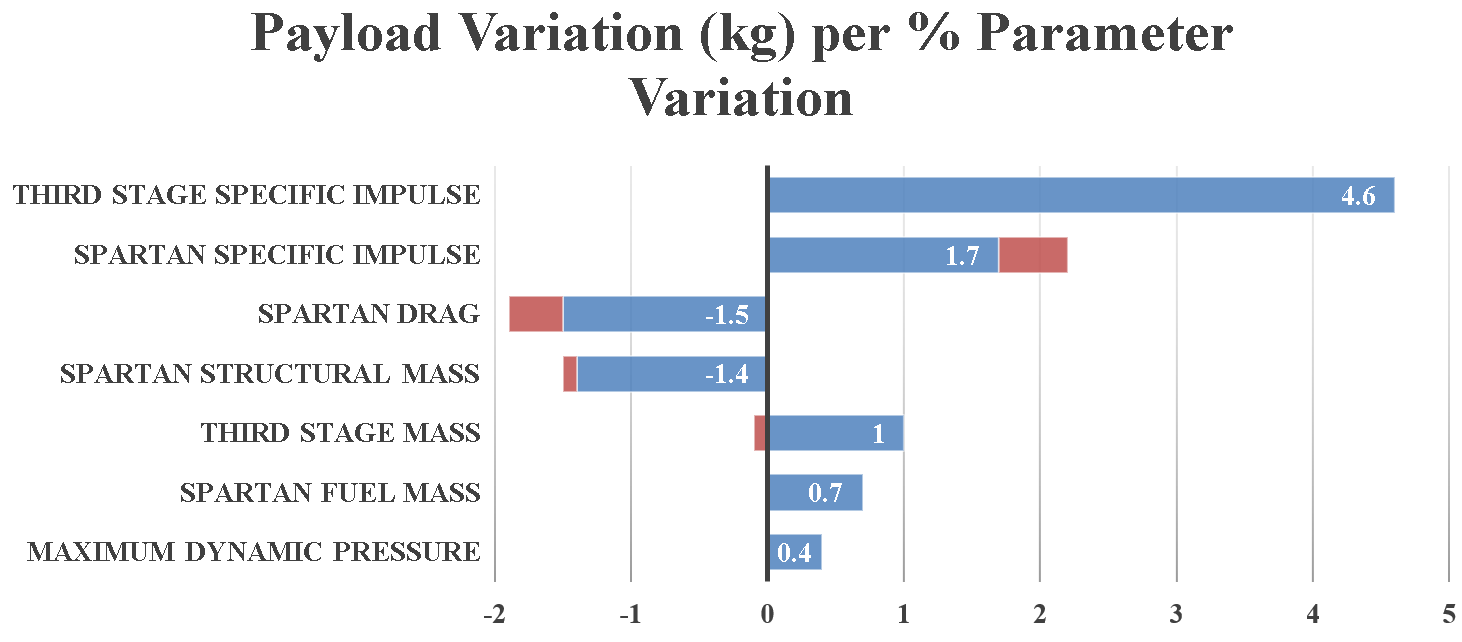
\includegraphics[width=0.99\linewidth]{figures/6_FlyBack/BarChart}
	\caption{The sensitivity of the key design parameters of the launch system, including SPARTAN fly-back. Red and green coloured areas indicate decreases or increases in the magnitude of sensitivity respectively, compared to the sensitivity study without SPARTAN fly-back in Section \ref{sec:comparisonNoReturn}.}
	\label{fig:BarChartreturn}
\end{figure}

The sensitivities of the launch system to a variety of design parameters have been presented in the preceding sections. Figure \ref{fig:BarChartreturn} shows a relative comparison of the payload-to-orbit sensitivity for each parameter which has been tested, by percentage. 
When the fly-back of the SPARTAN is included, the sensitivity of the launch system to the specific impulse, drag, and mass of the SPARTAN decreases.  
This is due to the fly-back of the SPARTAN partially offsetting the effects of variations in the performance of the SPARTAN. As the performance of the SPARTAN improves, the velocity at SPARTAN-third stage separation increases, however, so does the ground distance which the SPARTAN covers during its ascent. This means that effects which are beneficial to the payload-to-orbit result in a more challenging fly-back, in turn necessitating the SPARTAN to trade-off performance in order to successfully return to the initial launch site.

The sensitivity of the launch system to the maximum dynamic pressure is unchanged when fly-back is included. However, the slight decrease in the sensitivity of the launch system to the structural mass of the SPARTAN, to -1.4$\frac{\Delta kg}{\Delta\%m_{SPARTAN}}$, means that the potential beneficial effects of reducing the maximum dynamic pressure of the SPARTAN are reduced slightly. So long as the mass of the SPARTAN reduces by 28.3kg for each 1kPa reduction in the maximum dynamic pressure, the performance of the launch system will improve.

For the specific impulse of the SPARTAN to be increased, it is likely that the shape of the C-REST engines or forebody will need to be modified, or extra systems will need to be added. 
 The sensitivity of the launch system to the specific impulse of the SPARTAN is decreased significantly when the fly-back of the SPARTAN is included, to 1.7$\frac{\Delta kg}{\Delta\%I_{SP,SPARTAN}}$, a decrease of -0.5$\frac{\Delta kg}{\Delta\%I_{SP,SPARTAN}}$ (-22.7\%) compared to the sensitivity without fly-back. The sensitivity of the launch system to the SPARTAN's structural mass is also decreased, to -1.4$\frac{\Delta kg}{\Delta\%m_{SPARTAN}}$. Comparing these sensitivities, it is apparent that if the specific impulse of the SPARTAN can be increased by 1\% with less than 1.21\% (60.0kg) increase in the total mass of the SPARTAN, then the overall performance of the launch system will be improved.  
Similarly, the sensitivity of the launch system to variation in the drag of the SPARTAN is reduced, to -1.5$\frac{\Delta kg}{\Delta\%C_{d,SPARTAN}}$. Comparing this sensitivity with the sensitivity to the structural mass of the SPARTAN, it can be seen that if the specific impulse of the C-REST engines can be improved by 1\%, while increasing the drag of the SPARTAN by less than 1.13\% due to shape variation, that the overall performance change will be beneficial. 
The decreased sensitivity of the launch system performance to the structural mass of the SPARTAN, along with the unchanged fuel mass sensitivity, means that so long as 1kg of fuel mass can be added with less than 1.59kg of structural mass added, the performance of the launch system will improve. Additionally, the decreased sensitivity of the launch system to the drag of the SPARTAN means that so long as 1kg of fuel can be added to the SPARTAN, with a drag increase of less than 0.030\%, then the maximum payload-to-orbit will increase. 
Comparing the increased third stage mass sensitivity, of 1$\frac{\Delta kg}{\Delta\%m_{3}}$, with the decreased SPARTAN drag sensitivity, shows that if the size of the third stage can be increased so that the third stage mass increases by 1kg while the fuselage of the SPARTAN varied so that the increase in SPARTAN drag is less than 0.020\%, the maximum payload-to-orbit will be improved. 





\section{Summary}

In this chapter, the maximum payload-to-orbit trajectory for a rocket-scramjet-rocket system has been calculated, with the inclusion of the fly-back of the SPARTAN scramjet-powered stage. It was found that it is possible for \PayloadToOrbitStandard kg of payload to be delivered to sun synchronous orbit, while successfully returning the scramjet-powered stage to the initial launch site. 
This return flight decreases the payload-to-orbit by -19.0kg (-10\%), but removes the need for the costly and time consuming transportation of the SPARTAN after launch, which would be necessary if landing at a downrange location.
During the return flight, the scramjet engines are powered on three times, in total using \returnFuelStandard kg of fuel for the return flight, 17.2\% of the SPARTAN's total fuel.

It was found that when the fly-back of the SPARTAN is included in the optimal trajectory calculation, the first stage of the launch system pitches in an easterly direction. 
The launch system exhibits a first stage-SPARTAN separation point of \firstsecondSeparationAltStandard km, an increase of 3.0km when compared to the maximum payload-to-orbit trajectory with no fly-back, and a trajectory angle of \firstsecondSeparationgammaStandard $^\circ$, an increase of 2.5$^\circ$. 
This higher separation point serves to increase the exergy efficiency of the first stage, to \firstExergyEffStandard \%$\eta$, an increase of +0.308\%$\eta$ (+4.9\%) when compared to the maximum payload-to-orbit trajectory with no fly-back.
In addition to increasing the exergy efficiency of the first stage, the higher first stage-SPARTAN separation serves to increase the altitude of the SPARTAN at the beginning of its trajectory. The SPARTAN banks heavily immediately after release, and descends, allowing for the heading angle to change rapidly. The SPARTAN maintains a high bank angle throughout its trajectory, executing a banking manoeuvre, and staying close to its maximum dynamic pressure. 
This banking manoeuvre decreases the exergy efficiency of the SPARTAN by -0.729\%$\eta$ (-15.4\%), but also reduces the ground distance necessary for the return of the SPARTAN, decreasing the amount of fuel necessary for fly-back, and increasing the overall efficiency of the SPARTAN. 
At the end of its acceleration, the SPARTAN was found to exhibit a pull-up manoeuvre before the separation of the third stage, in a similar fashion to the maximum payload-to-orbit trajectory with no fly-back. 

The fly-back of the SPARTAN is found to be separated into three stages; an initial turn, a boost phase, and an approach. 
The initial turn takes place immediately after separation, and consists of the SPARTAN banking heavily in order to manoeuvre the heading angle back towards the initial launch site. 
During the boost-skip phase the SPARTAN exhibits multiple `skipping' manoeuvres. These skipping manoeuvres have been shown in previous literature to extend the flight range of hypersonic vehicles\cite{Moshman2014,Darby2011,Toso2015,Tetlow1992}, and serve to reduce the amount of fuel used during the fly-back.
In addition, the skipping manoeuvres allow the scramjet engines to be powered on at the points where the specific impulse of the C-REST engines are highest, maximising the performance of the SPARTAN, and minimising the fuel necessary for return. 
During the approach phase, the trajectory of the SPARTAN is smoothed, and the SPARTAN glides to the landing point. 
 The optimal trajectory terminates when SPARTAN reaches 1km altitude at a velocity of 120m/s. After this point, it is assumed that the SPARTAN lands on a traditional runway.  
This result indicates that it is feasible to return a hypersonic launch vehicle from a high Mach number separation, to its initial launch site.  

The sensitivity of the launch system to various design parameters has been investigated. 
The payload-to-orbit sensitivity of the launch system to variations in the specific impulse, drag and structural mass of the SPARTAN was found to decrease when fly-back is included, compared to the sensitivity study with no fly-back. This decreased sensitivity indicates that the fly-back of the SPARTAN offsets some of the payload-to-orbit variation due to changes in these parameters. 

